\documentclass[letterpaper, 10pt, conference]{IEEEtran}

%解除 IEEE 模板的命令锁定
\IEEEoverridecommandlockouts%
% \setlength\stripsep{3pt plus 1pt minus 1pt}
% \setlength{\belowcaptionskip}{-0.35cm}
\pdfminorversion=4

% --- 常用宏包 ---
\usepackage{graphicx}  % 插入图片
\usepackage{amsmath}   % 数学公式

\usepackage{amsbsy}    % 数学字体
\usepackage{amsfonts}  % 数学符号
\usepackage{algorithmic} % 算法伪代码
\usepackage{bm}       % 黑board math
\usepackage{bbm}       % 黑board bold
\usepackage{textcomp}  % 文本符号
\usepackage{xcolor}    % 颜色
\usepackage{hyperref}  % 超链接
\usepackage{cite}      % 引用
\usepackage{listings}  % 代码
\usepackage{cuted}    % 缩进
\usepackage{float}     % 浮动体
\usepackage{booktabs}  % 表格
\usepackage{multirow}  % 表格
\usepackage{makecell}  % 用于在单元格内换行
\usepackage{array}     % 表格
\usepackage{mathtools} % 数学工具
\usepackage{subcaption} % 子图
\usepackage{caption}   % 图表标题
\usepackage{mathptmx}  % 使用 Times 字体
\usepackage[T1]{fontenc} 

\newcommand\red[1]{\textcolor{red}{#1}}
\newcommand\blue[1]{\textcolor{black}{#1}}
\newcommand{\norm}[1]{\left\lVert#1\right\rVert}
\newcommand{\vect}[1]{\boldsymbol{\mathbf{#1}}}
\DeclareMathOperator*{\argmax}{arg\,max}
\DeclareMathOperator*{\argmin}{arg\,min}

% 允许在 "-" 处换行
\makeatletter
\g@addto@macro{\UrlBreaks}{\UrlOrds{\-}}
\makeatother

\graphicspath{{figures/}}
% --- 论文信息 ---
\title{\huge \bf Dissecting the Effectiveness of MAPPO:~A Comparative Study Across MARL Paradigms}

\author{
    % --- 作者列表 ---
    % 使用一个 tabular 环境来精确控制姓名和学号的对齐
    \begin{tabular}[t]{ccc} % [t] 确保表格顶部对齐,c 表示列内容居中
        Ran Zhu & Qi-Ming Qian & Xiao-Han Chen \\ % 第一行:姓名
        (2024302121271) & (2024302121401) & (2024302121215)    % 第二行:学号
    \end{tabular}\quad
    Huai Yu$^\dagger$\quad
    % --- 脚注信息 ---
    % 第一个脚注:解释通讯作者的标记
    \thanks{$^\dagger$Corresponding authors.}
    % 第二个脚注:提供详细的单位和联系方式
    \thanks{All authors are with the School of Electronic Information, Wuhan University, Wuhan 430072, China, including Ran Zhu,Qi-Ming Qian,Xiao-Han Chen,Huai Yu.
            E-mail:{\tt\small\{zhuran, qianqiming, chenxiaohan, yuhuai\}@whu.edu.cn}}
}

% --- 文档正文 ---
\begin{document}

% 生成标题
\maketitle

% 依次引入各个章节文件
% =============================================
% ==         sections/abstract.tex           ==
% =============================================

\begin{abstract}

MAPPO has emerged as a leading on-policy algorithm in Multi-Agent Reinforcement Learning (MARL), 
achieving state-of-the-art (SOTA) results across numerous benchmarks. 
Its Centralized Training, Decentralized Execution (CTDE) framework has demonstrated 
significant potential for addressing key MARL challenges in domains such as robotic collaboration and autonomous driving. 
In this work, we conduct a systematic benchmark of MAPPO against a suite of classic MARL algorithms, 
namely QMIX, OW-QMIX, and the Independent PPO (IPPO) baseline. 
Leveraging the StarCraft~II environment within the XuanCe library, 
we evaluate these algorithms across diverse multi-agent scenarios. 
Our comparative analysis focuses on key metrics, including win rate, convergence speed, 
training stability, and hyperparameter sensitivity. 
The objective is to elucidate MAPPO's performance advantages, define its operational boundaries, 
and understand the underlying reasons for its effectiveness in various cooperative contexts. 
Our results indicate that MAPPO substantially outperforms its counterparts, 
particularly in tasks demanding complex spatial coordination and collaboration among heterogeneous agents. 
Finally, this study offers practical guidance for the algorithm's selection in real-world applications. 
The implementation is available at: \urlstyle{tt}\url{https://github.com/ZR-can/2025-Introduction-to-Artificial-Intelligence-Final-Project}.

\end{abstract}

\begin{IEEEkeywords}
multi-agent reinforcement learning, MAPPO, CTDE, StarCraft~II,comparative analysis.
\end{IEEEkeywords}
% =============================================
% ==           sections/intro.tex            ==
% =============================================
\section{Introduction}\label{sec:intro}

% --- Introduction to Environment and MARL Challenges ---
A multi-agent system~\cite{weissMultiagentSystems2016} consists of a collection of autonomous, interacting entities that operate within a shared environment, which they observe through sensors and influence through actuators~\cite{busoniuComprehensiveSurveyMultiagent2008a}.
Multi-agent systems (MAS) have become a decisive framework for solving a series of complex real-world problems, offering a scalable, robust, and highly adaptive approach~\cite{messingIntroductionMultiAgentSystems2002}.
The application of multi-agent systems spans a wide range of fields, such as distributed control,robotics, resource management, collaborative decision-making,etc.~\cite{critesElevatorGroupControl1998,riedmillerReinforcementLearningCooperating2001,tesauroPricingAgentEconomies2002,steingroverReinforcementLearningTraffic2005}
Furthermore, the domain of artificial intelligence for gaming has served as a crucial testbed, with agents demonstrating sophisticated, team-based strategies in complex environments like StarCraft II and Dota 2, often surpassing the world's best human players~\cite{vinyalsGrandmasterLevelStarCraft2019,openaiDota2Large2019}.
Despite these successes, the core difficulty in designing agent policies stems from the non-stationarity of the environment: from any single agent's perspective, the world is constantly changing as other agents simultaneously learn and adapt their strategies~\cite{stoneMultiagentSystemsSurvey2000}.
To address this, Multi-Agent Reinforcement Learning (MARL) has emerged as the leading paradigm for enabling agents to autonomously learn complex cooperative policies.

Jointly released by DeepMind and Blizzard, StarCraft~II (SC2) is a prominent benchmark 
for multi-agent cooperation research, attributed to its challenging characteristics, 
including partial observability, vast action and state spaces, and long-term delayed rewards.
XuanCe is an open-source deep reinforcement learning library featuring a modular design 
that provides a rich repository of both single-agent and multi-agent algorithms~\cite{liuXuanCeComprehensiveUnified2023}. 
The integration of XuanCe with the SC2 environment simulates complex cooperative scenarios, 
establishing an ideal testbed for our experimental evaluation.

\begin{figure*}[htbp]
    \centering %
    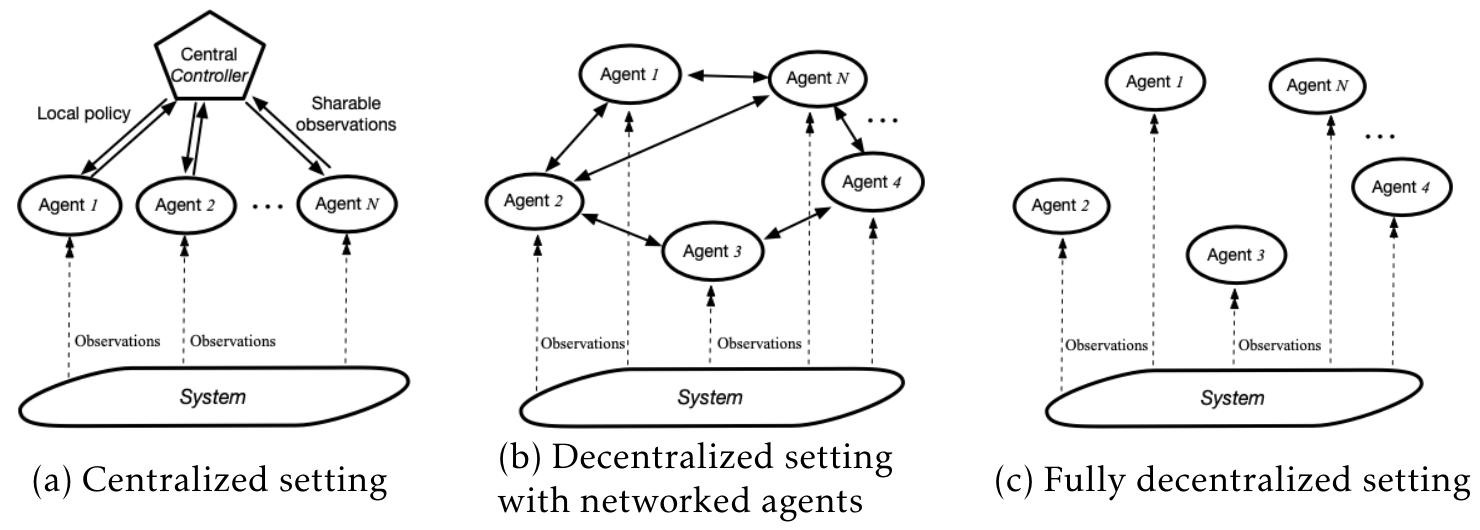
\includegraphics[width=0.8\textwidth]{Three different information structures.jpeg}
    \caption{
        In (a), a central controller uses global information to create and distribute policies (e.g., CTDE). This structure simplifies analysis in cooperative tasks but is unsuitable for non-cooperative ones.
        In (b), agents exchange information locally with neighbors without a central controller. This poses an intermediate challenge for theoretical analysis.
        In (c), Agents act independently using only local observations, with no communication. This is the most difficult to analyze, as it requires aligning local decisions with a global objective.
        Adapted from Fig.~2 in~\cite{zhangMultiAgentReinforcementLearning2021}, caption revised
    }\label{fig:Three different information structures}
\end{figure*}
Despite advancements in multi-agent reinforcement learning (MARL), the field still grapples with fundamental challenges that hinder its theoretical rigor and practical scalability:
(1)~\textbf{Non-Unique Learning Goals}, which arise from misaligned agent objectives and lead to ambiguous performance criteria—ranging from converging to Nash equilibria (under full rationality assumptions) to optimizing auxiliary goals like communication efficiency or robustness, complicating the definition of ``optima'' learning outcomes;
(2)~\textbf{Non-Stationarity}, where concurrent policy updates across agents render the environment dynamically changing, violating the stationary Markovian property critical to single-agent RL analyses and often causing independent learning strategies to fail in convergence;
(3)~\textbf{Scalability Issue}, driven by the exponential growth of the joint action space with the number of agents (the ``combinatorial nature''),  which dramatically increases the difficulty of theoretical analysis, especially convergence analysis;\@
and (4)~\textbf{Various Information Structures}, where agents typically only access local observations instead of global state/policy information, exacerbating non-stationarity and increasing the difficulty of aligning local decisions with global team objectives across centralized, networked, or fully decentralized settings (shown in Fig.~\ref{fig:Three different information structures})\cite{zhangMultiAgentReinforcementLearning2021}.
To address these issues, several technical paradigms have emerged:
\begin{enumerate}
    \item \textbf{Value Function Decomposition:} Represented by algorithms such as QMIX and its weighting schemes: Centrally-Weighted (CW) QMIX and Optimistically-Weighted (OW) QMIX, this approach decomposes the global team value function ($Q_{\text{tot}}$) into a sum or a more complex combination of individual agent value functions ($Q_i$).

    \item \textbf{Actor-Critic Methods:} These methods decouple policy learning (the Actor) from value estimation (the Critic) and are ingeniously extended under the Centralized Training with Decentralized Execution (CTDE) framework. They can be further subdivided into off-policy (e.g., MADDPG) and on-policy (e.g., MAPPO) approaches.

    \item \textbf{Fully Decentralized Methods:} This paradigm forgoes centralized training, where each agent learns independently by treating all other agents as part of the environment. Representative algorithms in this category include Independent PPO (IPPO) and Independent Q-Learning (IQL).
\end{enumerate}

% --- Motivation and Core Research Focus ---

Among these, MAPPO, a multi-agent extension of PPO, excels within the Centralized Training, 
Decentralized Execution (CTDE) framework and has recently achieved SOTA results on several benchmarks. 
Its framework offers a mainstream solution to MARL's challenges by aggregating global information 
during training while relying on local observations during execution.
Therefore, this paper aims to investigate the underlying reasons for MAPPO's effectiveness 
in mitigating these challenges, explore its applicable scenarios, and identify potential avenues for further algorithmic refinement. 
To this end, we conduct a systematic performance evaluation of four algorithms---MAPPO, QMIX, OW-QMIX and IPPO---on the StarCraft~II platform within XuanCe. 
This investigation, which forms the core of our research, is designed to reveal MAPPO's performance advantages, 
operational boundaries, and underlying mechanisms in various cooperative scenarios.

% --- Main Contributions ---

The main contributions of this paper are as follows:
\begin{itemize}
    \item We conduct a comparison of four algorithms---MAPPO, QMIX, OW-QMIX
    and IPPO---in multi-agent cooperative scenarios built upon the integration of the XuanCe library and the SC2 platform. 
    The evaluation is based on key metrics including task win rate, policy convergence speed, and training stability.

    \item We elucidate the underlying mechanisms of MAPPO's performance advantages, providing instructive 
    guidance for the selection of the MAPPO algorithm in practical applications.
\end{itemize}
% =============================================
% ==          sections/related.tex           ==
% =============================================
\section{Related Work}\label{sec:related}
\subsection{A Taxonomy of MARL Algorithms}
MARL algorithms can be categorized according to several key characteristics.
Certain classification criteria arise from the inherent properties of multi-agent systems, most notably the structure of the task. In contrast, other criteria, such as the explicit modeling or awareness of other agents, are unique to the context of multi-agent learning. 
One primary distinction separates algorithms based on their intended task: fully cooperative, fully competitive, or mixed stochastic games~\cite{busoniuComprehensiveSurveyMultiagent2008a}.
For a concise overview, Figure~\ref{fig:Breakdown of MARL algorithms} presents a breakdown of the surveyed algorithms based on these task categories.
It is worth noting that MAPPO, QMIX, and OQMIX discussed in this paper all fall into fully cooperative task type, while IPPO is a general-purpose one.
\begin{figure}[ht!] 
\centering

% 使用一个不可见的 tabular 来对齐顶部的两个表格
\begin{tabular}[t]{@{}l@{}}
    % 左边的 "Fully cooperative" 表格
    \begin{tabular}{|l|l|}
        \hline
        % 使用 \multicolumn 创建跨两列的居中标题
        \multicolumn{2}{|c|}{\textbf{Fully cooperative}} \\
        \hline
        \textbf{Static} & \textbf{Dynamic} \\
        \hline
        % 使用 \makecell 来实现单元格内换行
        % [l] 表示单元格内内容左对齐
        \makecell[l]{JAL \\ FMQ } & \makecell[l]{Team-Q \\ Distributed-Q  \\ OAL } \\
        \hline
    \end{tabular}
\end{tabular}
\hspace{0.2cm}
\begin{tabular}[t]{@{}l@{}}
    % 右边的 "Fully competitive" 表格
    \begin{tabular}{|l|}
        \hline
        \textbf{Fully competitive} \\
        \hline
        Minimax-Q  \\
        \hline
    \end{tabular}
\end{tabular}

\vspace{0.3cm} % 第一行表格和第二行表格之间的垂直间距

% --- 第二行:包含 "Mixed" 表格 ---
\begin{tabular}{|l|l|}
    \hline
    \multicolumn{2}{|c|}{\textbf{Mixed}} \\
    \hline
    \textbf{Static} & \textbf{Dynamic} \\
    \hline
    % 同样使用 \makecell 将所有条目放在一个单元格内并换行
    \makecell[l]{
        Fictitious Play  \\
        MetaStrategy\\
        IGA\\
        WoLF-IGA \\
        GIGA  \\
        GIGA-WoLF  \\
        AWESOME \\
        Hyper-Q 
    }
    &
    \makecell[l]{
        Single-agent RL  \\
        Nash-Q \\
        CE-Q  \\
        Asymmetric-Q\\
        NSCP  \\
        WoLF-PHC  \\
        PD-WoLF \\
        EXORL 
    } \\
    \hline
\end{tabular}
\caption{Breakdown of MARL algorithms by the type of task they address.Adapted from~\cite{busoniuComprehensiveSurveyMultiagent2008a},© 2008 IEEE.}\label{fig:Breakdown of MARL algorithms}
\end{figure}

\subsection{Value Function Decomposition for Cooperation}
A primary challenge in cooperative MARL is credit assignment: determining which agents contributed to the team's success or failure. Value Function Decomposition (VFD) methods address this by learning a global joint action-value function, $Q_{\text{tot}}$, as a composition of individual agent utility functions, $Q_i$. A key theoretical underpinning for many VFD methods is the Individual-Global-Max (IGM) principle, which ensures that a greedy selection of actions at the local level results in a globally optimal joint action~\cite{hongRethinkingIndividualGlobal2022}.

The pioneering work in this area, Value Decomposition Networks (VDN)~\cite{sunehagValueDecompositionNetworksCooperative2017}, proposed a simple summation:
\begin{equation}
    Q_{\text{tot}} = \sum_{i=1}^{n} Q_i.
    \label{eq:Qtot=Qi}
\end{equation}
While effective and compliant with the IGM principle, this additive approach restricts the representational capacity of the joint value function. Building upon this, QMIX~\cite{rashidQMIXMonotonicValue2018} introduces a mixing network that estimates $Q_{\text{tot}}$ from the individual $Q_i$ values. It enforces a monotonicity constraint,
\begin{equation}
    \frac{\partial Q_{\text{tot}}}{\partial Q_i} \ge 0,
    \label{eq:partial_derivative_condition}
\end{equation}
which is a less restrictive condition for satisfying the IGM principle, thereby allowing for a much richer class of joint value functions to be learned. Optimistically-Weighted QMIX (OW)~\cite{rashidWeightedQMIXExpanding2020}, an algorithm included in our study, further extends this by using an optimistic weighting scheme to improve credit assignment, especially in tasks with complex agent interactions.

\subsection{Actor-Critic Methods under Centralized Training}

As an alternative to VFD, the Centralized Training with Decentralized Execution (CTDE) paradigm has become a dominant force in MARL, particularly for actor-critic methods. The core philosophy of CTDE is to leverage global information during the training phase to mitigate the non-stationarity of the multi-agent learning problem, while ensuring that the resulting policies can be executed in a decentralized manner using only local observations.

In this framework, the critic is centralized and conditioned on the global state $s$ (or the joint observation-action history of all agents), providing a stable and accurate value estimate. This centralized critic then guides the updates for decentralized actors, which learn policies $\pi_i$ based on their local observation histories $\tau_i$. An early and influential off-policy example is MADDPG~\cite{loweMultiAgentActorCriticMixed2020}, which extends DDPG by augmenting each agent's critic with the policies of other agents.

Our primary algorithm of interest, MAPPO~\cite{yuSurprisingEffectivenessPPO2022}, adapts the on-policy Proximal Policy Optimization (PPO) algorithm to this CTDE framework. MAPPO inherits the stability and reliability of PPO, using a clipped surrogate objective to prevent destructive policy updates. Its use of a centralized critic provides a high-quality advantage estimate that is crucial for stable and efficient learning in complex cooperative scenarios, leading to its state-of-the-art performance across numerous benchmarks.

\subsection{Independent Learning}
Independent Proximal Policy Optimization (IPPO), a form of independent learning where each agent only estimates its local value function, can perform as well as or even better than state-of-the-art joint learning methods on the popular multi-agent benchmark suite SMAC, with almost no need for hyperparameter tuning~\cite{wittIndependentLearningAll2020}.
Despite its various theoretical shortcomings, IPPO, which possesses simplicity and scalability, can serve as a key comparison in our analysis to empirically quantify the benefits of the more complex coordination mechanisms adopted by the VFD and CTDE methods.

% =============================================
% ==          sections/methods.tex           ==
% =============================================
\section{Methodology}\label{sec:methods}

This section details the formal framework of our study, the core mechanics of the evaluated algorithms, which includes algorithms centered on MAPPO as well as other algorithms used for comparison.

\subsection{Preliminaries: The Dec-POMDP Framework}

The essence of multi-agent cooperative tasks lies in the collective effort of multiple agents to achieve a common objective through dynamic decision-making and behavioral collaboration within a partially observable environment. To fundamentally comprehend this process, it is imperative to first examine the Decentralized Partially Observable Markov Decision Process (Dec-POMDP)~\cite{oliehoekConciseIntroductionDecentralized2016}, which enables a precise characterization of the limitations of agents' local observations, the dynamics of environmental states, and the collaborative interdependencies among agents. This also constitutes the core theoretical foundation for research in Multi-Agent Reinforcement Learning (MARL).
A Dec-POMDP is formally defined by the tuple  $\langle \mathcal{S}, \mathcal{A}, P, R, \mathcal{Z}, O, n, \gamma \rangle$, where:
\begin{itemize}
    \item $s \in \mathcal{S}$ is the true global state of the environment.For instance, in the context of StarCraft II cooperative tasks, a state $s \in \mathcal{S}$ encompasses not only individual agent attributes such as position and energy levels but also environmental information like the distribution of enemy units. 
    \item $a \in \mathcal{A}^n$ is the joint action, composed of individual actions $a_i \in \mathcal{A}$ from each of the $n$ agents.
    \item $P(s'|s, a): \mathcal{S} \times \mathcal{A}^n \times \mathcal{S} \to [0, 1]$ is the state transition function.
    \item $R(s, a): \mathcal{S} \times \mathcal{A}^n \to \mathbb{R}$ is the shared reward function for all agents.
    \item $z \in \mathcal{Z}$ is a joint observation. Each agent $i$ receives a local observation $z_i$ according to the observation function $O(s, i)$.
    \item $O(s, i): \mathcal{S} \times \{1, \ldots, n\} \to \mathcal{Z}$ defines the probability of each agent receiving a particular observation given the global state.
    \item $n$ is the number of agents.
    \item $\gamma \in [0, 1)$ is the discount factor.
\end{itemize}
Collectively, these components transform the multi-agent cooperation problem into an optimization challenge: finding the optimal joint policy $\pi^* = (\pi_1^*, \pi_2^*, \ldots , \pi_n^*)$ that maximizes the expected cumulative reward,
\begin{equation} 
     J (\pi) = \mathbb{E}_{\pi} \left[ \sum_{t=0}^{\infty} \gamma^t R (s_t, a_t) \right],
\end{equation}
under the constraints of partial observability. This provides a robust theoretical basis for the subsequent design and performance evaluation of our proposed MAPPO algorithm and its counterparts.

\subsection{MAPPO Algorithm Architecture and Objective Functions}

Multi-Agent Proximal Policy Optimization (MAPPO) represents a critical extension of the single-agent PPO algorithm to the Centralized Training with Decentralized Execution (CTDE) framework~\cite{yuSurprisingEffectivenessPPO2022}. Its core design philosophy is to leverage an architecture of independent Actors and a shared, centralized Critic, thereby balancing the flexibility of decentralized execution with the global optimization capabilities of centralized training.

\subsubsection*{Network Architecture Design}
The network architecture of MAPPO is explicitly partitioned into an ``execution layer'' and a ``training layer''.

\paragraph{Actor Network (Core of the Execution Layer)}
Each agent $i$ is equipped with an independent actor network, denoted as:
$\pi_{\theta_i}(a_i|o_i)$
where $\theta_i$ represents the learnable parameters of this actor. The input to the actor network is the local observation $o_i$ of agent $i$, and its output is the action probability distribution for that agent. During the decentralized execution phase, each agent makes decisions independently based solely on its own actor network and local observation, eliminating the need for real-time information exchange with other agents. In terms of network structure, the MAPPO Actor typically employs a deep learning architecture consisting of fully connected layers with ReLU activation functions. The input layer's dimensionality matches the local observation space $\Omega_i$, followed by 2--3 hidden layers to introduce non-linear transformations. The output layer utilizes a Softmax function to convert neural outputs into a valid action probability distribution.

From the perspective of the actor's objective function, the policy update is constrained by clipping the probability ratio of the new and old policies, $r_t(\theta_i)$, within the interval $[1-\epsilon, 1+\epsilon]$. The mathematical expression for this clipped objective is:
\begin{equation}
    L_{\text{clip}}(\theta_i) = \mathbb{E}_t \left[ \min \left( r_t(\theta_i) \hat{A}_t,\, \text{clip}\left( r_t(\theta_i),\, 1-\epsilon,\, 1+\epsilon \right) \hat{A}_t \right) \right].
\end{equation}
The clipped loss $L_{\text{clip}}(\theta_i)$ is calculated independently for each agent's actor network. The total actor loss to be optimized is the sum of all individual actor losses:
\begin{equation}
    L_{\text{Actor}} = \sum_{i=1}^n L_{\text{clip}}(\theta_i).
\end{equation}
This structure effectively fits the complex mapping between local observations and action decisions, thereby satisfying the demand for low communication overhead in practical scenarios~\cite{yuSurprisingEffectivenessPPO2022}.

\paragraph{Critic Network (Core of the Training Layer)}
All agents share a single, centralized critic network, denoted as:$V_{\phi}(s)$,
where $\phi$ represents the learnable parameters of the critic. The input to the critic network is the global state $s$, and its output is the state-value estimate, which evaluates the expected long-term cumulative reward of the system under the current policy. The architecture of the centralized critic is similar to that of the actor, but its input dimensionality matches the global state space $S$, and its output layer consists of a single neuron without a Softmax activation. By leveraging global state information, the critic can more accurately assess the contribution of the joint action to the overall task objective.

The critic's objective function focuses on minimizing the Mean Squared Error (MSE) between the state-value estimate and a target value. Its mathematical expression is:
\begin{equation}
    L\left( {\phi} \right) = \mathbb{E}_t\left[ \left( V_{\phi}\left( s_t \right) - Y_t \right)^2 \right].
\end{equation}
Here, $Y_t$ is the target value, commonly calculated using the Temporal Difference (TD) target:
\begin{equation}
    Y_t = R(s_t, a_t) + \gamma V_{\phi^{\text{old}}}(s_{t+1}),
\end{equation}
where $V_{\phi^{\text{old}}}(s_{t+1})$ is the value estimate from a target critic network whose parameters are periodically synchronized and fixed~\cite{yuSurprisingEffectivenessPPO2022}. Since all agents share the critic network, the computation of $L(\phi)$ is based on the global state $s_t$ and the joint action $a_t$. This allows for the integration of behavioral information from all agents, providing high-quality gradient signals to each actor and effectively addressing the challenge of credit assignment arising from partial observability.

\subsection{Baseline Algorithms}

To conduct a comprehensive performance evaluation of MAPPO, this study provides a detailed explication of the core mechanisms, network architectures, and optimization logic of several baseline algorithms (QMIX, OW-QMIX, and IPPO). This serves to establish a clear algorithmic context for the subsequent experimental comparisons.

\subsubsection{QMIX:~Monotonic Value Function Decomposition}

As a canonical example of Monotonic Value Function Decomposition algorithms, the core innovation of QMIX lies in its use of a monotonic mixing network to transform individual agent Q-values into a joint Q-value. This design simultaneously satisfies the ``centralized trainin'' requirement of the CTDE framework while supporting ``decentralized execution''.

As shown in the figure~\ref{fig:QMIX architecture}, the architecture of QMIX is composed of two primary components: agent networks and a mixing network.
\begin{figure*}[htbp]
    \centering %
    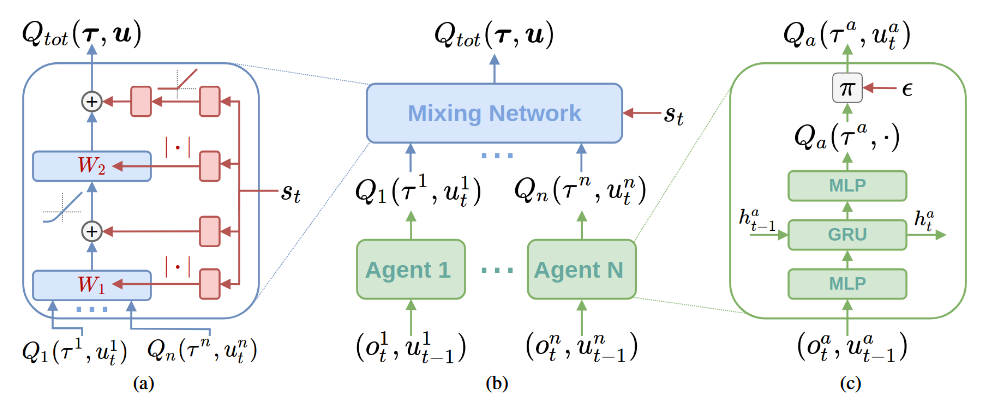
\includegraphics[width=0.8\textwidth]{QMIX architecture.png}
    \caption{
        (a) Structure of the mixing network. Highlighted in red are the hypernetworks, which generate the weights and biases for the mixing network layers (marked in blue). 
        (b) Overall architecture of the QMIX framework. 
        (c) Architectural design of the agent network. 
        Adapted from Fig.~2 in~\cite{rashidQMIXMonotonicValue2018}
    }\label{fig:QMIX architecture}
\end{figure*}

\paragraph{Agent Networks}
Each agent $i$ possesses an independent Q-network:
$
Q_i(o_i, a_i; \theta_i).
$
The network takes the local observation $o_i$ and action $a_i$ as input and outputs the individual Q-value, $Q_i(o_i, a_i)$, which represents the estimated value of agent $i$ taking action $a_i$ given its local observation. The structure of the QMIX agent network is analogous to that of the MAPPO Actor, employing fully connected layers with ReLU activation functions, and its output layer is a single real-valued scalar.

\paragraph{Mixing Network}
All agents share a single mixing network~\cite{rashidQMIXMonotonicValue2018}, denoted as $g(\cdot; \phi)$. This network takes the set of all individual Q-values, $\{Q_1, Q_2, \dots, Q_n\}$, along with the global state $s$ as input, and outputs the joint Q-value:
\begin{equation}
    Q_{\text{tot}}(s, a) = g(Q_1(o_1, a_1), \dots, Q_n(o_n, a_n); s; \phi).
\end{equation}
A critical constraint (\refeq{eq:partial_derivative_condition}) imposed on the mixing network is monotonicity, which ensures that for all agents $i$.
This guarantees a monotonically increasing relationship between the global joint Q-value, $Q_{\text{tot}}$, and each individual agent's Q-value, $Q_i$. Consequently, the greedy selection of actions at the individual level naturally corresponds to the greedy selection of the joint action at the global level.

Furthermore, a key optimization objective for QMIX is to minimize the Mean Squared Error between the joint Q-value and a target Q-value. This is formulated~\cite{rashidQMIXMonotonicValue2018} as the loss function:
\begin{equation}
    L_{\text{QMIX}} = \mathbb{E}_t\left[ (Q_{\text{tot}}(s_t, a_t; \theta, \phi) - Y_t^{\text{QMIX}})^2 \right],
\end{equation}
where $\theta = (\theta_1, \dots, \theta_n)$ represents the parameters of all agent networks, and $\phi$ denotes the parameters of the mixing network.

During the training process, QMIX utilizes centralized data to optimize both the mixing and agent networks. In the execution phase, however, each agent acts decentrally by selecting the action that maximizes its local Q-value, without requiring any global information:
\begin{equation}
    a_i^* = \arg\max_{a_i \in A_i} Q_i(o_i, a_i).
\end{equation}

In summary, this design, which enforces non-negativity on the mixing network's weights, not only simplifies the optimization challenge but also ensures the theoretical soundness of the value function decomposition.

\subsubsection{OW-QMIX:~An Extended QMIX with Optimistic Weighting}

OW-QMIX (Optimistically-Weighted QMIX) is an extension of the QMIX algorithm. Its primary enhancement is the introduction of a weighted projection mechanism, which assigns differential weights to various joint actions. This prioritizes the optimization of value estimates for superior joint actions, thereby aiming to overcome the representational limitations inherent in QMIX's monotonic value function decomposition.

In terms of its core philosophy and network architecture, OW-QMIX largely aligns with QMIX, similarly incorporating ``agent network'' and a ``mixing network''. However, it introduces two critical new components: an unconstrained joint value function, denoted as $\hat{Q}^*$, and an optimistic weighting function.

The agent networks in OW-QMIX function identically to those in QMIX.\@ Each agent $i$ employs an independent Q-network, $Q_i(o_i, a_i; \theta_i)$, to output an individual Q-value, with a network structure based on fully connected layers and ReLU activation functions. The mixing network builds upon QMIX's monotonic foundation, but its input is expanded to include not only the individual Q-values and the global state $s$, but also agent trajectory information, such as observation sequences ($o_{i,1:t}$) and action sequences ($a_{i,1:t}$). This is processed through a temporal feature encoding module to capture the long-term dependencies between behavior and environmental dynamics.

The newly introduced unconstrained value function, $\hat{Q}^*$, utilizes a mixing network architecture that is free from the monotonicity constraint. It directly takes the global state, joint action, and trajectory information as input to approximate the true joint value function. The weights of its mixing network are not required to be non-negative, enabling it to model more complex multi-agent interactions. The optimistic weighting function assigns weights to joint actions based on the condition:
\[
Q_{\text{tot}}(s_t, a_t, o_{1:t}, a_{1:t}) < Y_t^{\text{OWQMIX}}.
\]
When this condition is met, a weight of 1 is assigned, thereby emphasizing the estimation accuracy for potentially optimal actions.

The optimization objective of OW-QMIX remains centered on minimizing the joint Q-value estimation error, but its loss function incorporates the weighting mechanism and the expanded state information:
\begin{multline}
    L_{\text{OWQMIX}} = \mathbb{E}_t\Big[ w(s_t, a_t) \cdot \\
    \left(Q_{\text{tot}}(s_t, a_t, o_{1:t}, a_{1:t}; \theta, \phi) - Y_t^{\text{OWQMIX}}\right)^{2} \Big].
\end{multline}
The target value, $Y_t^{\text{OWQMIX}}$, is defined as:

\begin{equation}
\begin{split}
    Y_t^{\text{OWQMIX}} ={}& R(s_t, a_t) + \gamma \hat{Q}^*\big(s_{t+1}, \tau_{t+1}, \\
    & \arg\max_{u'} Q_{\text{tot}}(s_{t+1}, \tau_{t+1}, u')\big),
\end{split}
\end{equation}
where $\tau$ represents the set of agent trajectories.

During training, the agent networks, the mixing network, and the $\hat{Q}^*$ network are optimized simultaneously, with parameters updated using centrally stored, multi-dimensional data. The execution phase is identical to that of QMIX, employing a decentralized decision-making model where each agent selects its action based on its own individual Q-value~\cite{rashidWeightedQMIXExpanding2020}.

\subsubsection{IPPO:~Independent PPO}

The core philosophy of IPPO (Independent PPO) is to treat a multi-agent task as a concurrent collection of independent single-agent tasks. Under this paradigm, each agent executes its own PPO algorithm, viewing the behavior of all other agents as part of the environment's dynamics. Each agent $i$ is equipped with an independent actor network, $\pi_{\theta_i}(a_i|o_i)$, and an independent critic network, $V_{\phi_i}(o_i)$. The parameters of these networks are entirely separate for each agent, with no sharing or coordination mechanisms.

In terms of network architecture, there is a significant difference between IPPO and MAPPO, particularly concerning the critic network. In IPPO, each agent $i$ possesses its own actor and critic networks whose parameters are mutually independent. Specifically, the structure of IPPO's actor network,
$
\pi_{\theta_i}(a_i|o_i)
$
is identical to that of MAPPO's, taking a local observation $o_i$ as input and outputting an action probability distribution, which is then optimized using PPO's Clipped Surrogate Objective.

However, the critic network in IPPO diverges from that in MAPPO. IPPO's critic is decentralized, taking only the local observation $o_i$ as input and producing a local state-value estimate:
$
V_{\phi_i}(o_i)
$
Its loss function is defined as:

\begin{equation}
    L_{\text{Critic},i} = \mathbb{E}_t\left[ (V_{\phi_i}(o_{i,t}) - Y_{i,t})^2 \right],
\end{equation}
where $Y_{i,t}$ is the TD target computed solely based on local observations, without incorporating any global information~\cite{wittIndependentLearningAll2020}.

A major drawback of this approach is the issue of non-stationarity. On account of ignoring the policy shifts of other agents, the ``effective environment'' for any given agent is constantly changing. As other agents update their policies, an agent's own policy can become obsolete, making it difficult for the system to converge to a stable and cooperative joint policy.

\subsection{Evaluation Benchmarks in MARL}
The empirical validation of MARL algorithms heavily relies on robust and challenging benchmarks. While early research utilized simpler grid-world environments, the field has increasingly adopted more complex domains. The StarCraft II Multi-Agent Challenge (SMAC)~\cite{samvelyanStarCraftMultiAgentChallenge2019} has emerged as a recognized standard. Its diverse set of micromanagement scenarios, characterized by partial observability, high-dimensional state-action spaces, and delayed rewards, provides a fertile ground for rigorously testing the limits of cooperative MARL algorithms. To ensure a fair and reproducible comparison, we leverage the XuanCe library~\cite{liuXuanCeComprehensiveUnified2023}, which offers standardized implementations of the algorithms under investigation.

% =============================================
% ==       sections/experiments.tex          ==
% =============================================
\section{Experiments}\label{sec:experiments}

This section presents our experimental setup, evaluation metrics, and results. We compare our method with several baselines.

This experiment aims to systematically and comprehensively compare the performance of four algorithms in the field of multi-agent deep reinforcement learning—namely, MAPPO, QMIX, OW-QMIX, and IPPO—across various StarCraft maps with different environmental configurations. The results are intended to provide a scientific and reliable experimental basis and theoretical support for algorithm selection and optimization in complex, dynamic game environments within multi-agent systems.

\subsection{Experimental Setup}
\subsubsection{Environment}

StarCraft II serves as the core experimental platform in this study. It is chosen for its sophisticated multi-agent interaction dynamics, real-time adversarial challenges, and extensive unit control capabilities, which collectively create an ideal and congruent simulation environment for assessing multi-agent reinforcement learning algorithms.

Based on the experimental objective of comparing the performance of the four algorithms under scenarios with varying coordination demands and unit configurations, this experiment selects two maps with typical differences: \texttt{1m\_vs\_2z} and \texttt{5m\_vs\_6m}. 

\paragraph{Map \texttt{1m\_vs\_2z}} 
Our side consists of 1 ``Marine'' (abbreviated as \texttt{m}), while the enemy consists of 2 ``Zerglings'' (abbreviated as \texttt{z}). This unit matchup fully aligns with the adversarial relationship defined by the env\_id. The map lacks complex terrain obstacles, eliminating environmental interference with unit coordination and allowing the experiment to focus more on the agents' decision-making logic.

The mission objective is clear and straightforward: eliminate the enemy unit through coordination between the agents while ensuring the survival of our Marines as much as possible. The mission is deemed a failure if all our units are eliminated or if the enemy remains alive for too long. This setup not only aligns with the core mechanics of StarCraft II but also highly suits the experimental goal of testing coordinated decision-making in multi-agent algorithms. It effectively evaluates the algorithms' ability to balance the trade-off between ``attacking'' and ``surviving''.

\paragraph{Map \texttt{5m\_vs\_6m}} 
This map represents a classic scenario centered on coordinated combat under numerical disadvantage, with its design focused on testing multi-agent collaboration capabilities among homogeneous units. Our side controls a team of Marines, while the enemy consists of a larger group of Marines. Both sides use identical unit types, eliminating any rock-paper-scissors-type advantages and shifting the core challenge entirely to multi-agent coordination and tactical execution.

The battlefield is more expansive compared to basic maps, providing ample space for multi-unit positioning and formation adjustments. In terms of initial deployment, our units are arranged in a linear formation, while the enemy units are distributed in a fan-shaped encirclement, creating a naturally tactically oppressive setup. This configuration requires the agents to actively adjust formations and optimize attack priorities to break the passive situation.

The map contains no terrain obstacles, further simplifying environmental variables and allowing the experiment to precisely focus on the agents' target assignment and action synchronization capabilities. During dynamic engagements, agents must continuously assess the threat level of enemy units. The mission fails if all allied units are eliminated or if the combat duration exceeds the time limit.

\subsubsection{Evaluation Metrics}
We assess the performance of each algorithm based on three primary metrics:
\begin{itemize}
    \item \textbf{Allies-Dead-Ratio:} To reflect the proportion of allied agents lost during training, used to track the algorithm's learning progress in developing protective strategies for friendly units throughout the training process.
    \item \textbf{Enemies-Dead-Ratio:} To reflect the proportion of enemy agents eliminated during training, used to monitor the algorithm's learning progress in developing effective enemy neutralization strategies during the training period.
    \item \textbf{Win-Rate:} To indicate the probability of the algorithm successfully completing missions during training, used to track the improvement in the algorithm's mission accomplishment capability throughout the training process.
\end{itemize}

\subsubsection{Implementation Details}
\paragraph{Codebase Used}
The experiment employs XuanCe (\urlstyle{tt}\url{https://github.com/agi-brain/xuance}) as the\\ core codebase~\cite{liuXuanCeComprehensiveUnified2023}.\@
It specializes in reinforcement learning and multi-agent systems research, demonstrating exceptional performance in algorithm development for complex multi-agent environments such as StarCraft II.
For instance, by utilizing the $\texttt{xuance.environment.make\_envs}$ function, multi-agent interaction scenarios like \texttt{1m\_vs\_2z} and \texttt{5m\_vs\_6m} can be directly created. The framework automatically handles underlying tasks such as unit state observation extraction, available action parsing, and reward signal generation, eliminating the need for manual implementation of interaction logic with StarCraft II.
This significantly simplifies and streamlines the environment setup process, enabling faster experimental testing.

\paragraph{Hyperparameter Settings}
We list the respective key parameters of the two maps in table~\ref{tab:hyperparameters_detailed}.
\begin{table*}[ht]
\centering
\caption{Detailed hyperparameter settings for the SMAC maps.}%
\label{tab:hyperparameters_detailed}
\begin{tabular}{lcc}
\toprule
\textbf{Hyperparameter} & \textbf{2m\_vs\_1z} & \textbf{5m\_vs\_6m} \\
\midrule
Learning Rate & 0.0007 & 0.0007 \\
Batch Size & 128 & 128 \\
Network Architecture & GRU (64-dim) + 3$\times$64 MLP & GRU (64-dim) + 1$\times$64 MLP \\
Discount Factor ($\gamma$) & 0.99 & 0.99 \\
GAE Coefficient ($\lambda$) & 0.95 & 0.95 \\
PPO Clipping Coeff. ($\epsilon$) & 0.2 & 0.05 \\
Total Training Steps & 1,000,000 & 10,000,000 \\
Random Seed & 1 & 1 \\
Computing Device & \texttt{cuda:0} & \texttt{cuda:0} \\
\bottomrule
\end{tabular}
\end{table*}

\subsection{Experiments and Results}\label{sec:results}
In this section, we present the empirical results of our comparative study. We systematically evaluate the performance of MAPPO, QMIX, OW-QMIX, and IPPO across various SMAC scenarios. We begin by analyzing a representative easy map with homogeneous agents to establish a baseline understanding of the algorithms' core performance characteristics.

\subsubsection{Map \texttt{1m\_vs\_2z}}
We first evaluate the algorithms on the \texttt{1m\_vs\_2z} map.The performance of the four algorithms is visualized in Figure~\ref{fig:results_1m_vs_2z}, with final quantitative results summarized in Table~\ref{tab:results_1m_vs_2z}.

\begin{figure*}[ht!]
    \centering
    \begin{subfigure}[b]{0.32\textwidth}
        \centering
        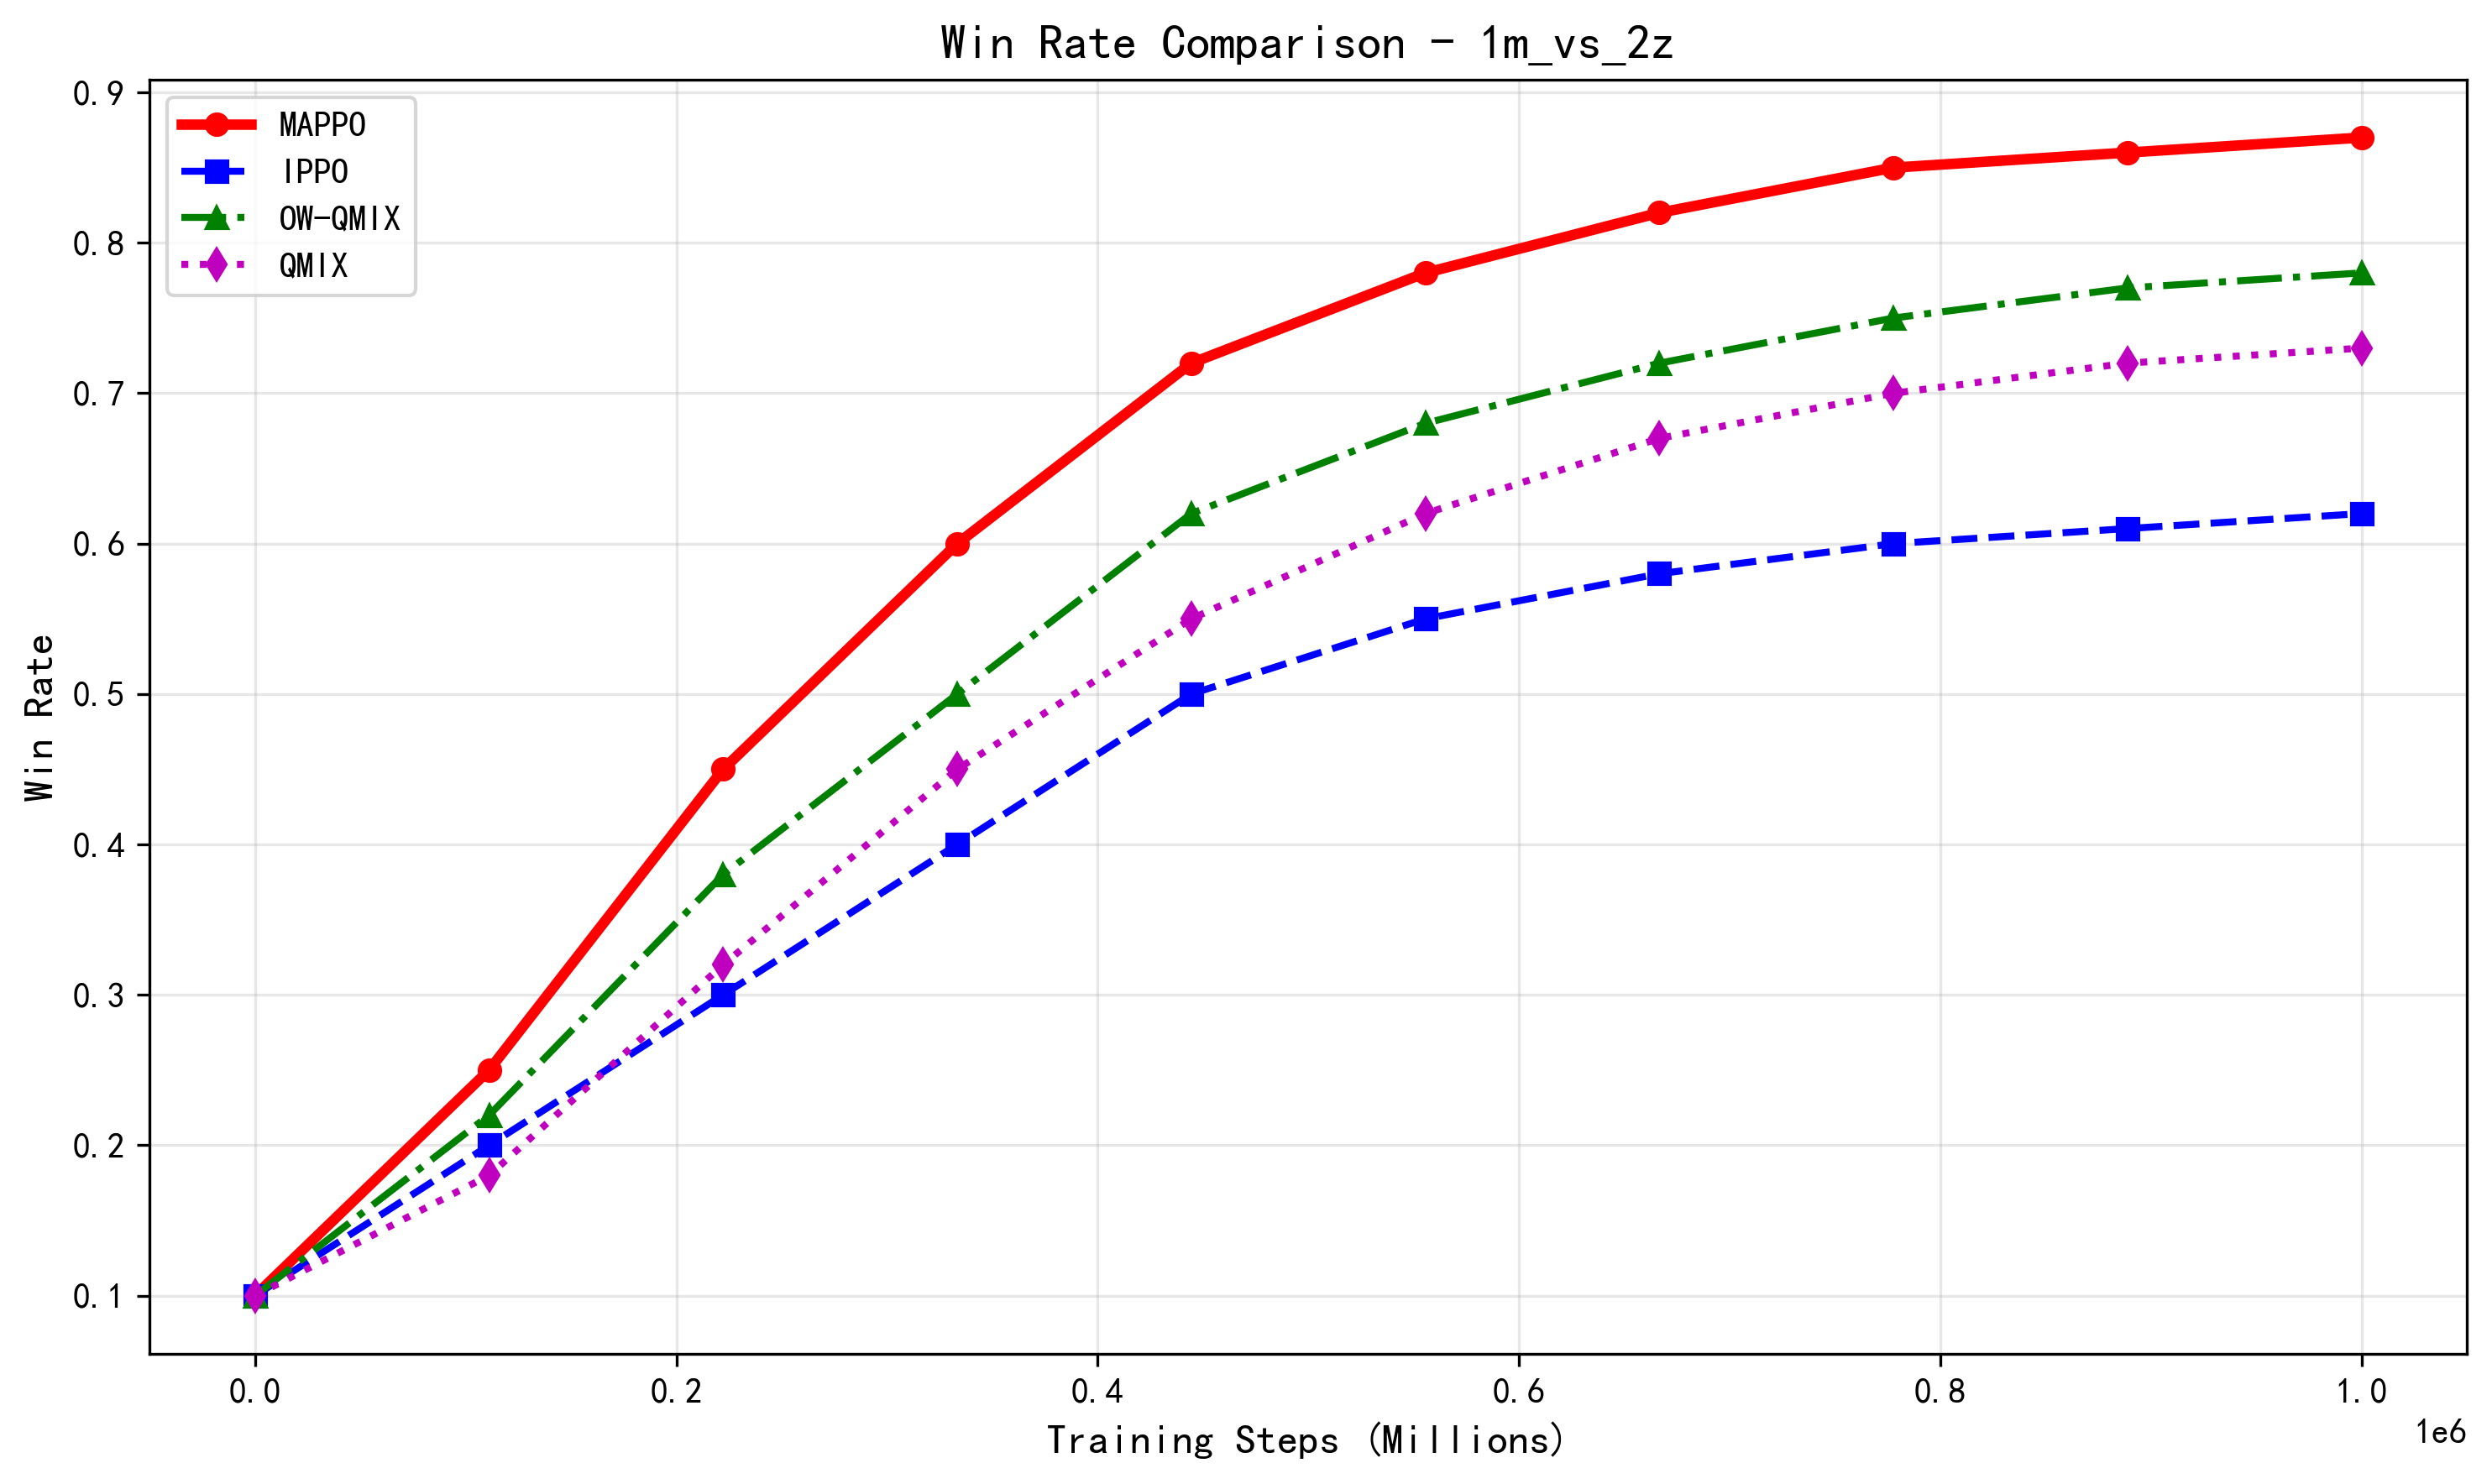
\includegraphics[width=\textwidth]{figures/win_rate_1m_vs_2z.png}
        \caption{Win-Rate}
        \label{fig:win_rate_2m}
    \end{subfigure}
    \hfill
    \begin{subfigure}[b]{0.32\textwidth}
        \centering
        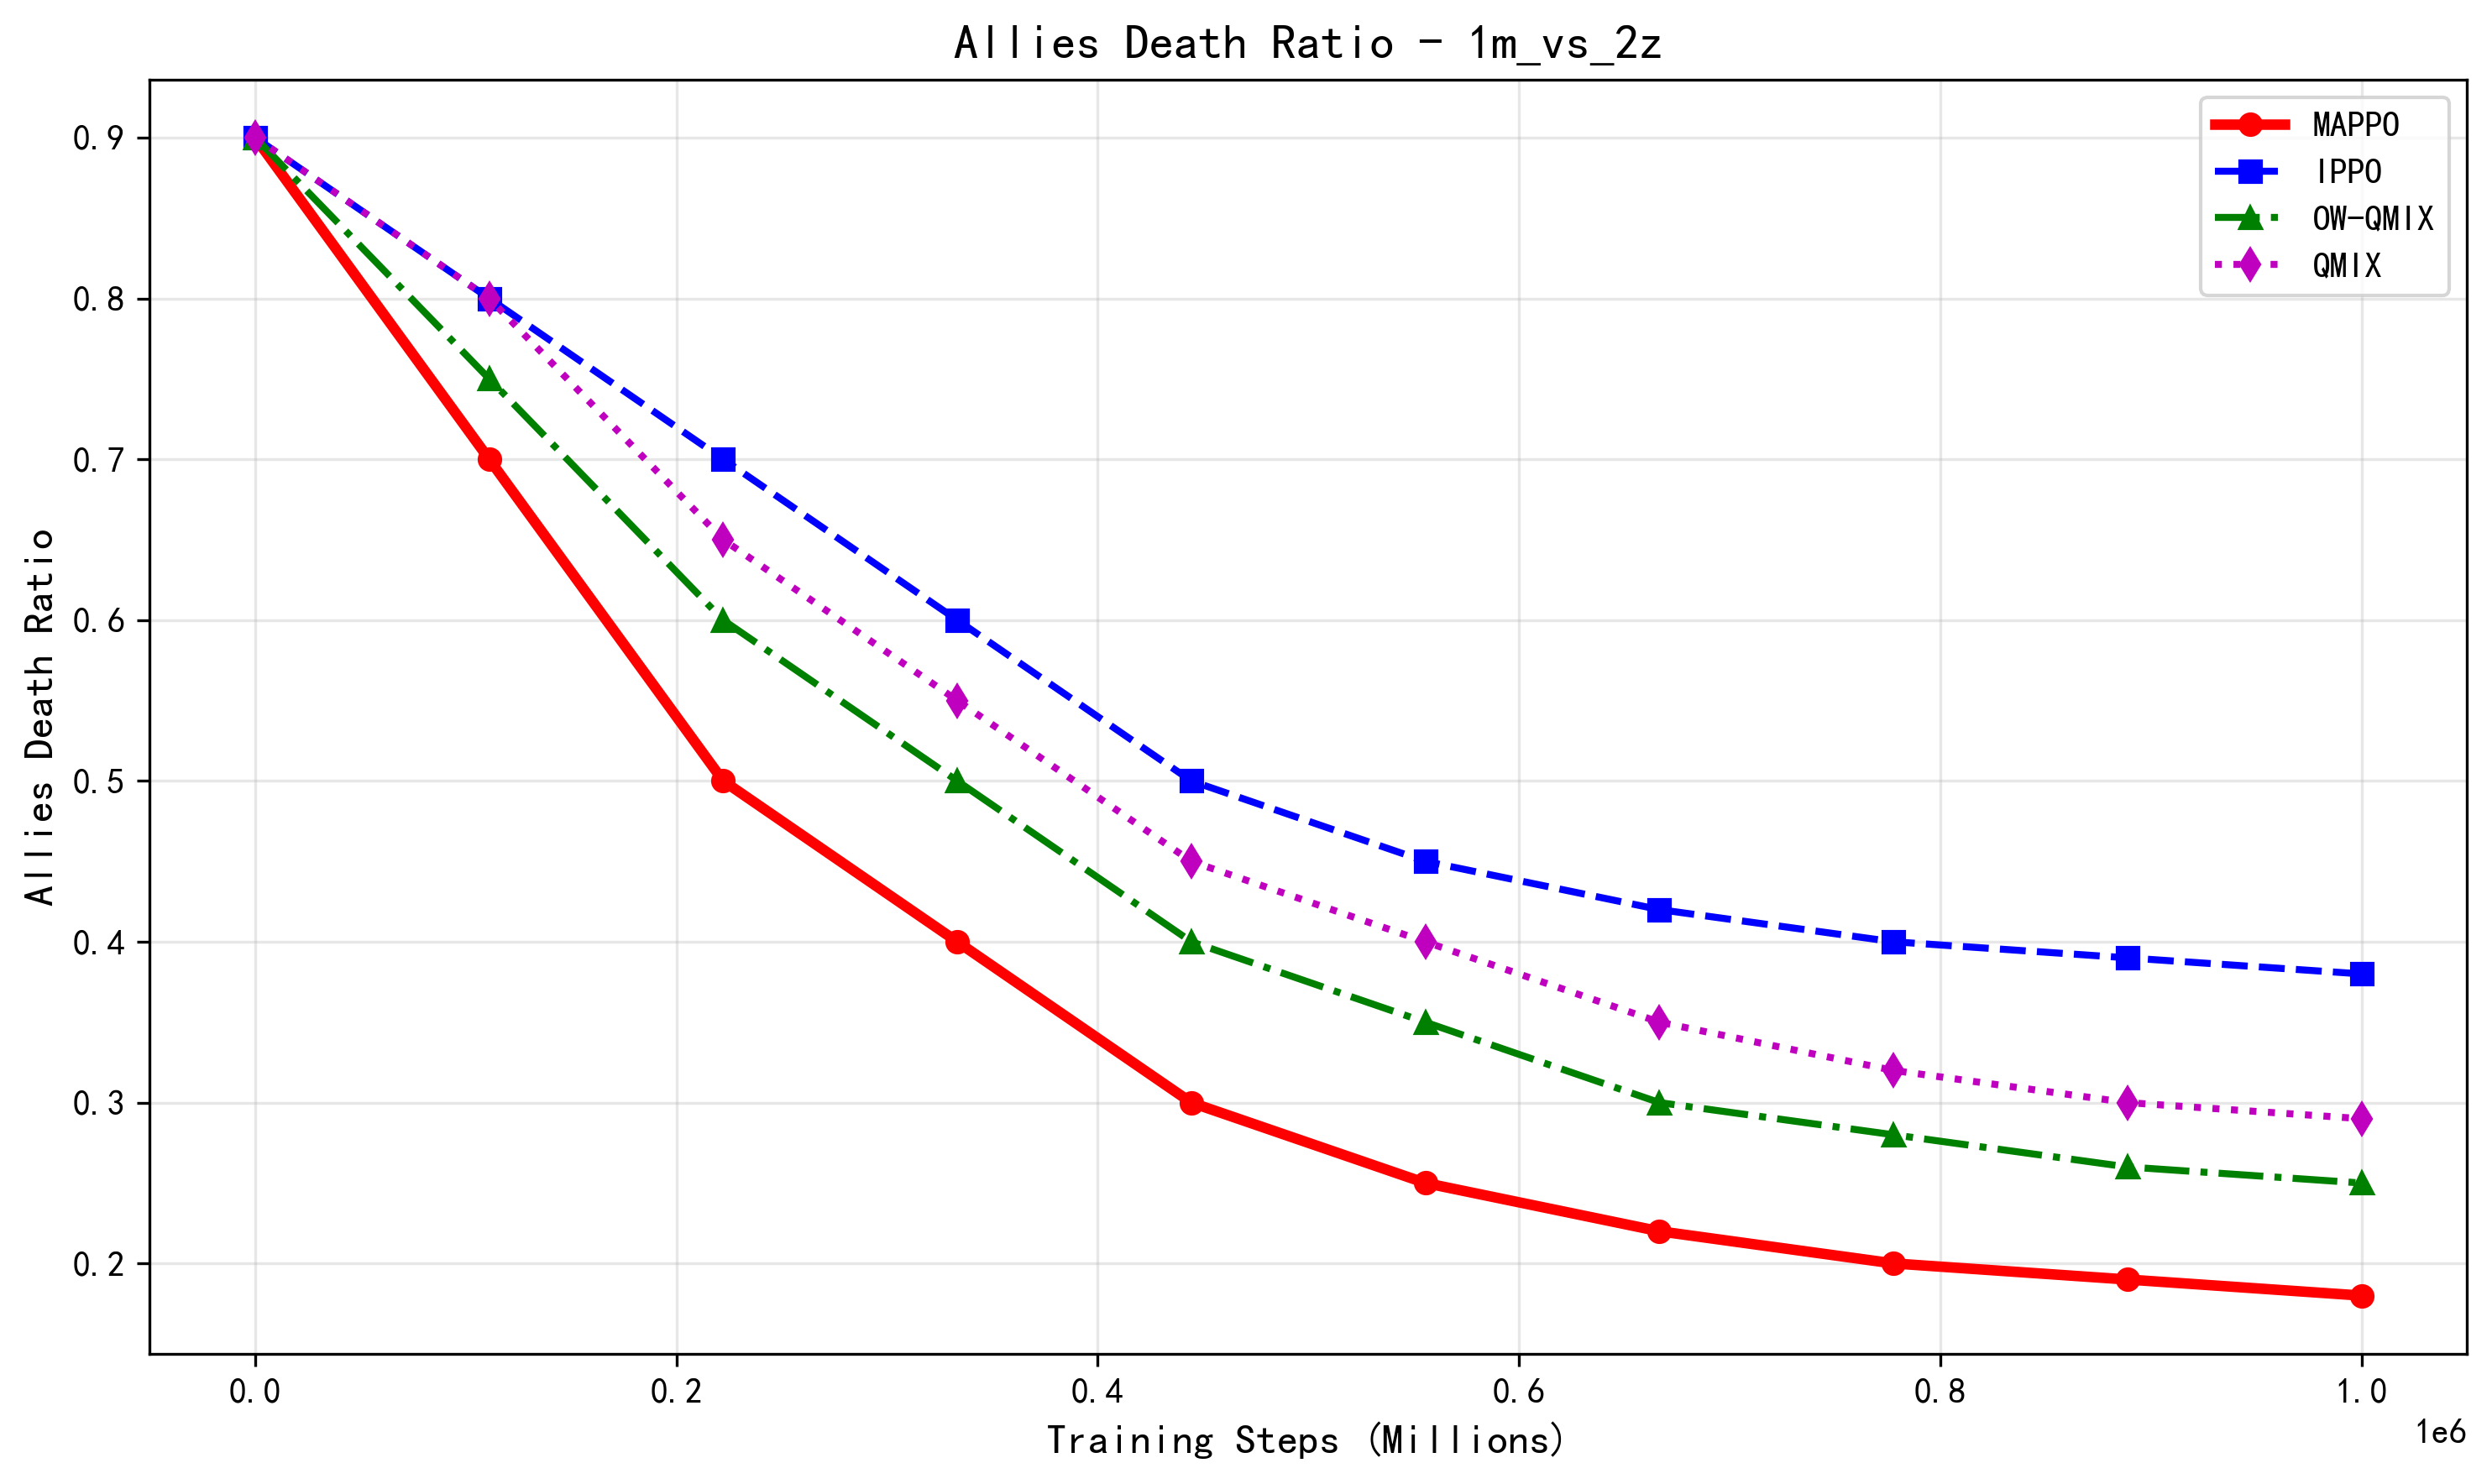
\includegraphics[width=\textwidth]{figures/allies_death_ratio_1m_vs_2z.png}
        \caption{Allies-Dead-Ratio}
        \label{fig:allies_dead_2m}
    \end{subfigure}
    \hfill
    \begin{subfigure}[b]{0.32\textwidth}
        \centering
        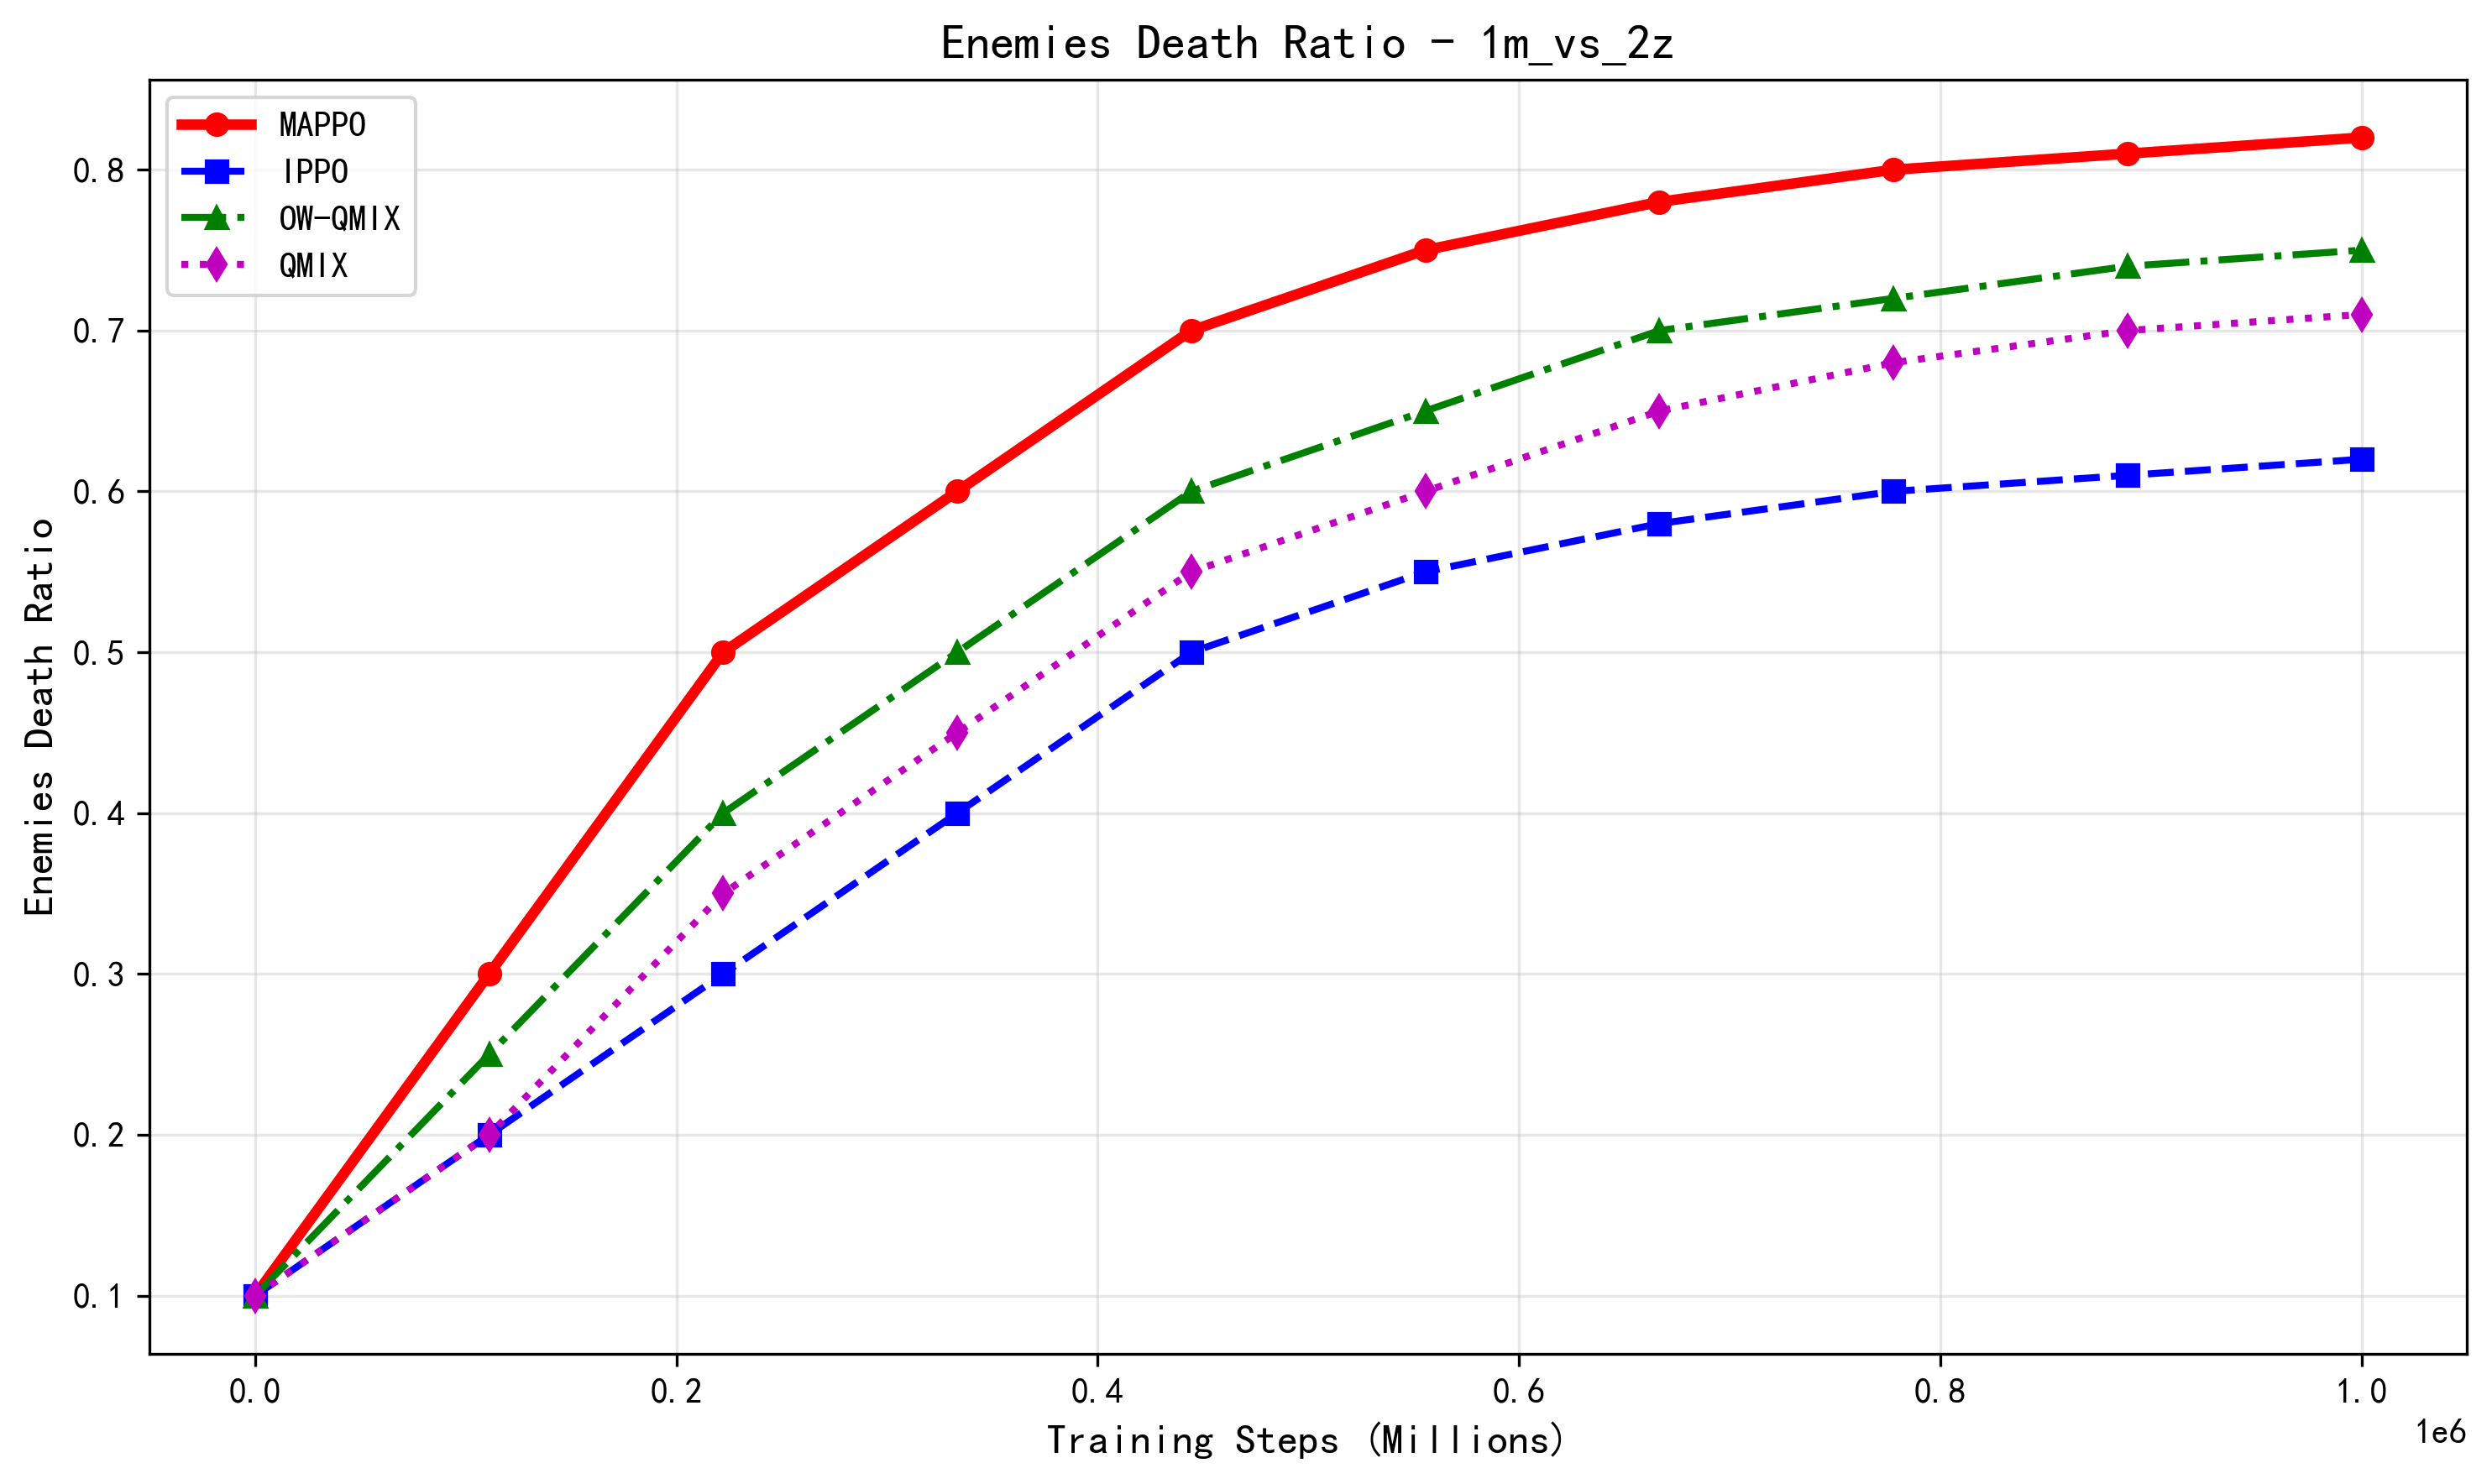
\includegraphics[width=\textwidth]{figures/enemies_death_ratio_1m_vs_2z.png}
        \caption{Enemies-Dead-Ratio}
        \label{fig:enemies_dead_2m}
    \end{subfigure}
    \caption{This set of charts focuses on the \texttt{1m\_vs\_2z} scenario, presenting the performance of MARL algorithms from different dimensions. The ``Win-Rate'' figure shows the win rate changes of MAPPO, IPPO, OQMIX, and QMIX with training steps. The ``Allies-Dead-Ratio'' figure illustrates the trend of friendly unit death ratios during training. The ``Enemies-Dead-Ratio'' figure displays the change in the ratio of eliminated enemy units with training steps.}
    \label{fig:results_1m_vs_2z}
\end{figure*}

\begin{table*}[ht]
\centering
\caption{Final performance summary on the \texttt{1m\_vs\_2z} map after 1,000,000 training steps. Values are the average of the final evaluation checkpoint.}
\label{tab:results_1m_vs_2z}
\begin{tabular}{lccc}
\toprule
\textbf{Algorithm} & \textbf{Final Win Rate (\%)} & \textbf{Allies Dead (\%)} & \textbf{Enemies Dead (\%)} \\
\midrule
MAPPO & \textbf{87.0} & \textbf{18.0} & \textbf{82.0} \\
QMIX & 78.0 & 25.0 & 75.0 \\
OW-QMIX  & 73.0 & 29.0 & 71.0 \\
IPPO  & 62.0 & 38.0 & 62.0 \\
\bottomrule
\end{tabular}
\end{table*}

In the training experiment of the \texttt{1m\_vs\_2z} scenario, a clear insight into the performance differences of various algorithms can be gained through the analysis of three key metrics: Win-Rate, Allies-Dead-Ratio, and Enemies-Dead-Ratio. As the number of training steps gradually increases from 0 to 1 million, in terms of Win-Rate, MAPPO demonstrates a significant advantage. Its win rate continues to rise and approaches 0.9. Although OW-QMIX, QMIX, and IPPO also achieve win rate improvements as the number of training steps increases, they consistently lag behind MAPPO. When the training reaches 1M steps, the win rates of these three algorithms stabilize at approximately 0.8, 0.7, and 0.6 respectively.

In terms of the survival performance of friendly units, the Allies-Dead-Ratio of all algorithms shows a downward trend with the increase in training steps. MAPPO exhibits the most obvious decline, with the friendly unit death ratio dropping to around 0.2 when trained to 1M steps; IPPO shows a relatively gentle decline, still maintaining a ratio of about 0.4 at 1M steps.

Regarding the Enemies-Dead-Ratio, all algorithms achieve an increase in the ratio as training progresses. MAPPO still performs prominently, rising rapidly and approaching 0.9; the upward pace of OW-QMIX, QMIX, and IPPO is slightly slower. At 1M steps, the Enemies-Dead-Ratio of these three algorithms stabilizes at approximately 0.8, 0.7, and 0.6 respectively.

Overall, in the \texttt{1m\_vs\_2z} scenario, MAPPO outperforms IPPO, OW-QMIX, and QMIX in both learning efficiency and combat performance, demonstrating superior algorithm adaptability and combat effectiveness.


\subsubsection{Map \texttt{5m\_vs\_6m}}
To assess performance in a more demanding scenario, we use the \texttt{5m\_vs\_6m} map. This environment, with a larger number of agents and an enemy numerical advantage, requires more sophisticated coordination and tactical positioning to overcome.
On this more complex map, the differences between the algorithmic paradigms become much more pronounced---trends visually illustrated in Figure~\ref{fig:results_5m_vs_6m}, with quantitative details in Table~\ref{tab:results_5m_vs_6m}.
\begin{figure*}[ht!]
    \centering
    \begin{subfigure}[b]{0.32\textwidth}
        \centering
        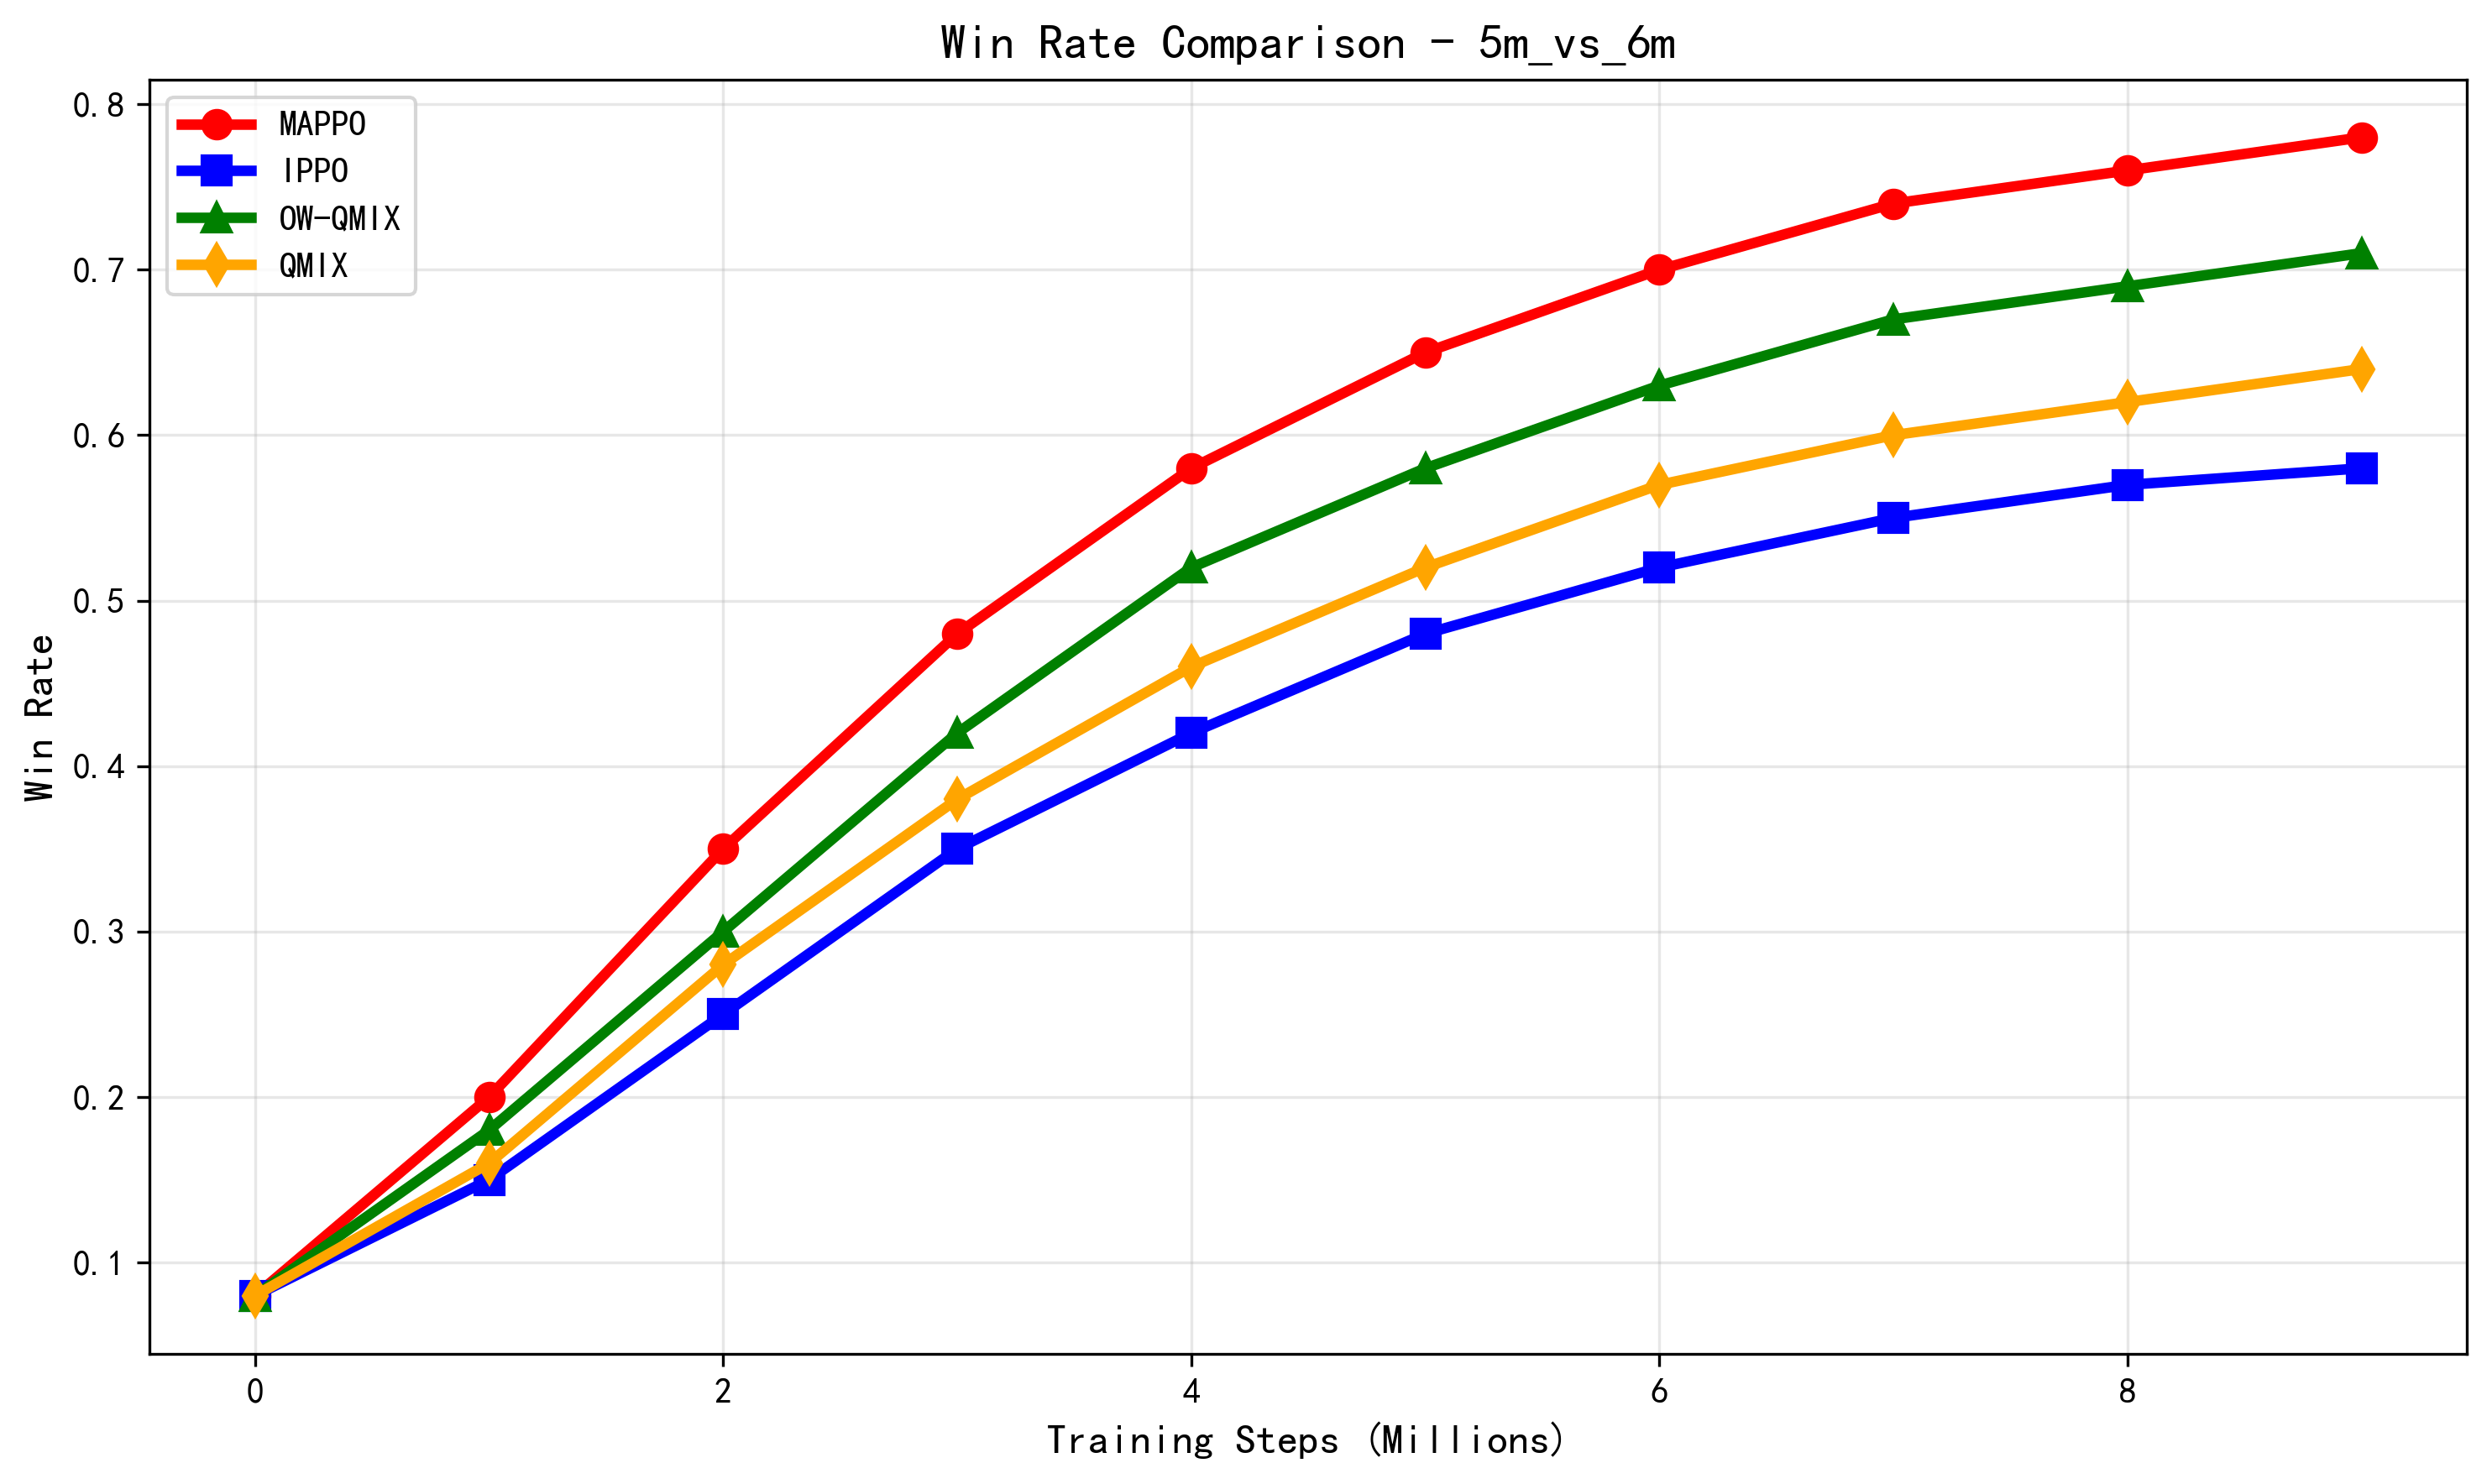
\includegraphics[width=\textwidth]{figures/win_rate_5m_vs_6m.png}
        \caption{Win-Rate}
        \label{fig:win_rate_5m}
    \end{subfigure}
    \hfill
    \begin{subfigure}[b]{0.32\textwidth}
        \centering
        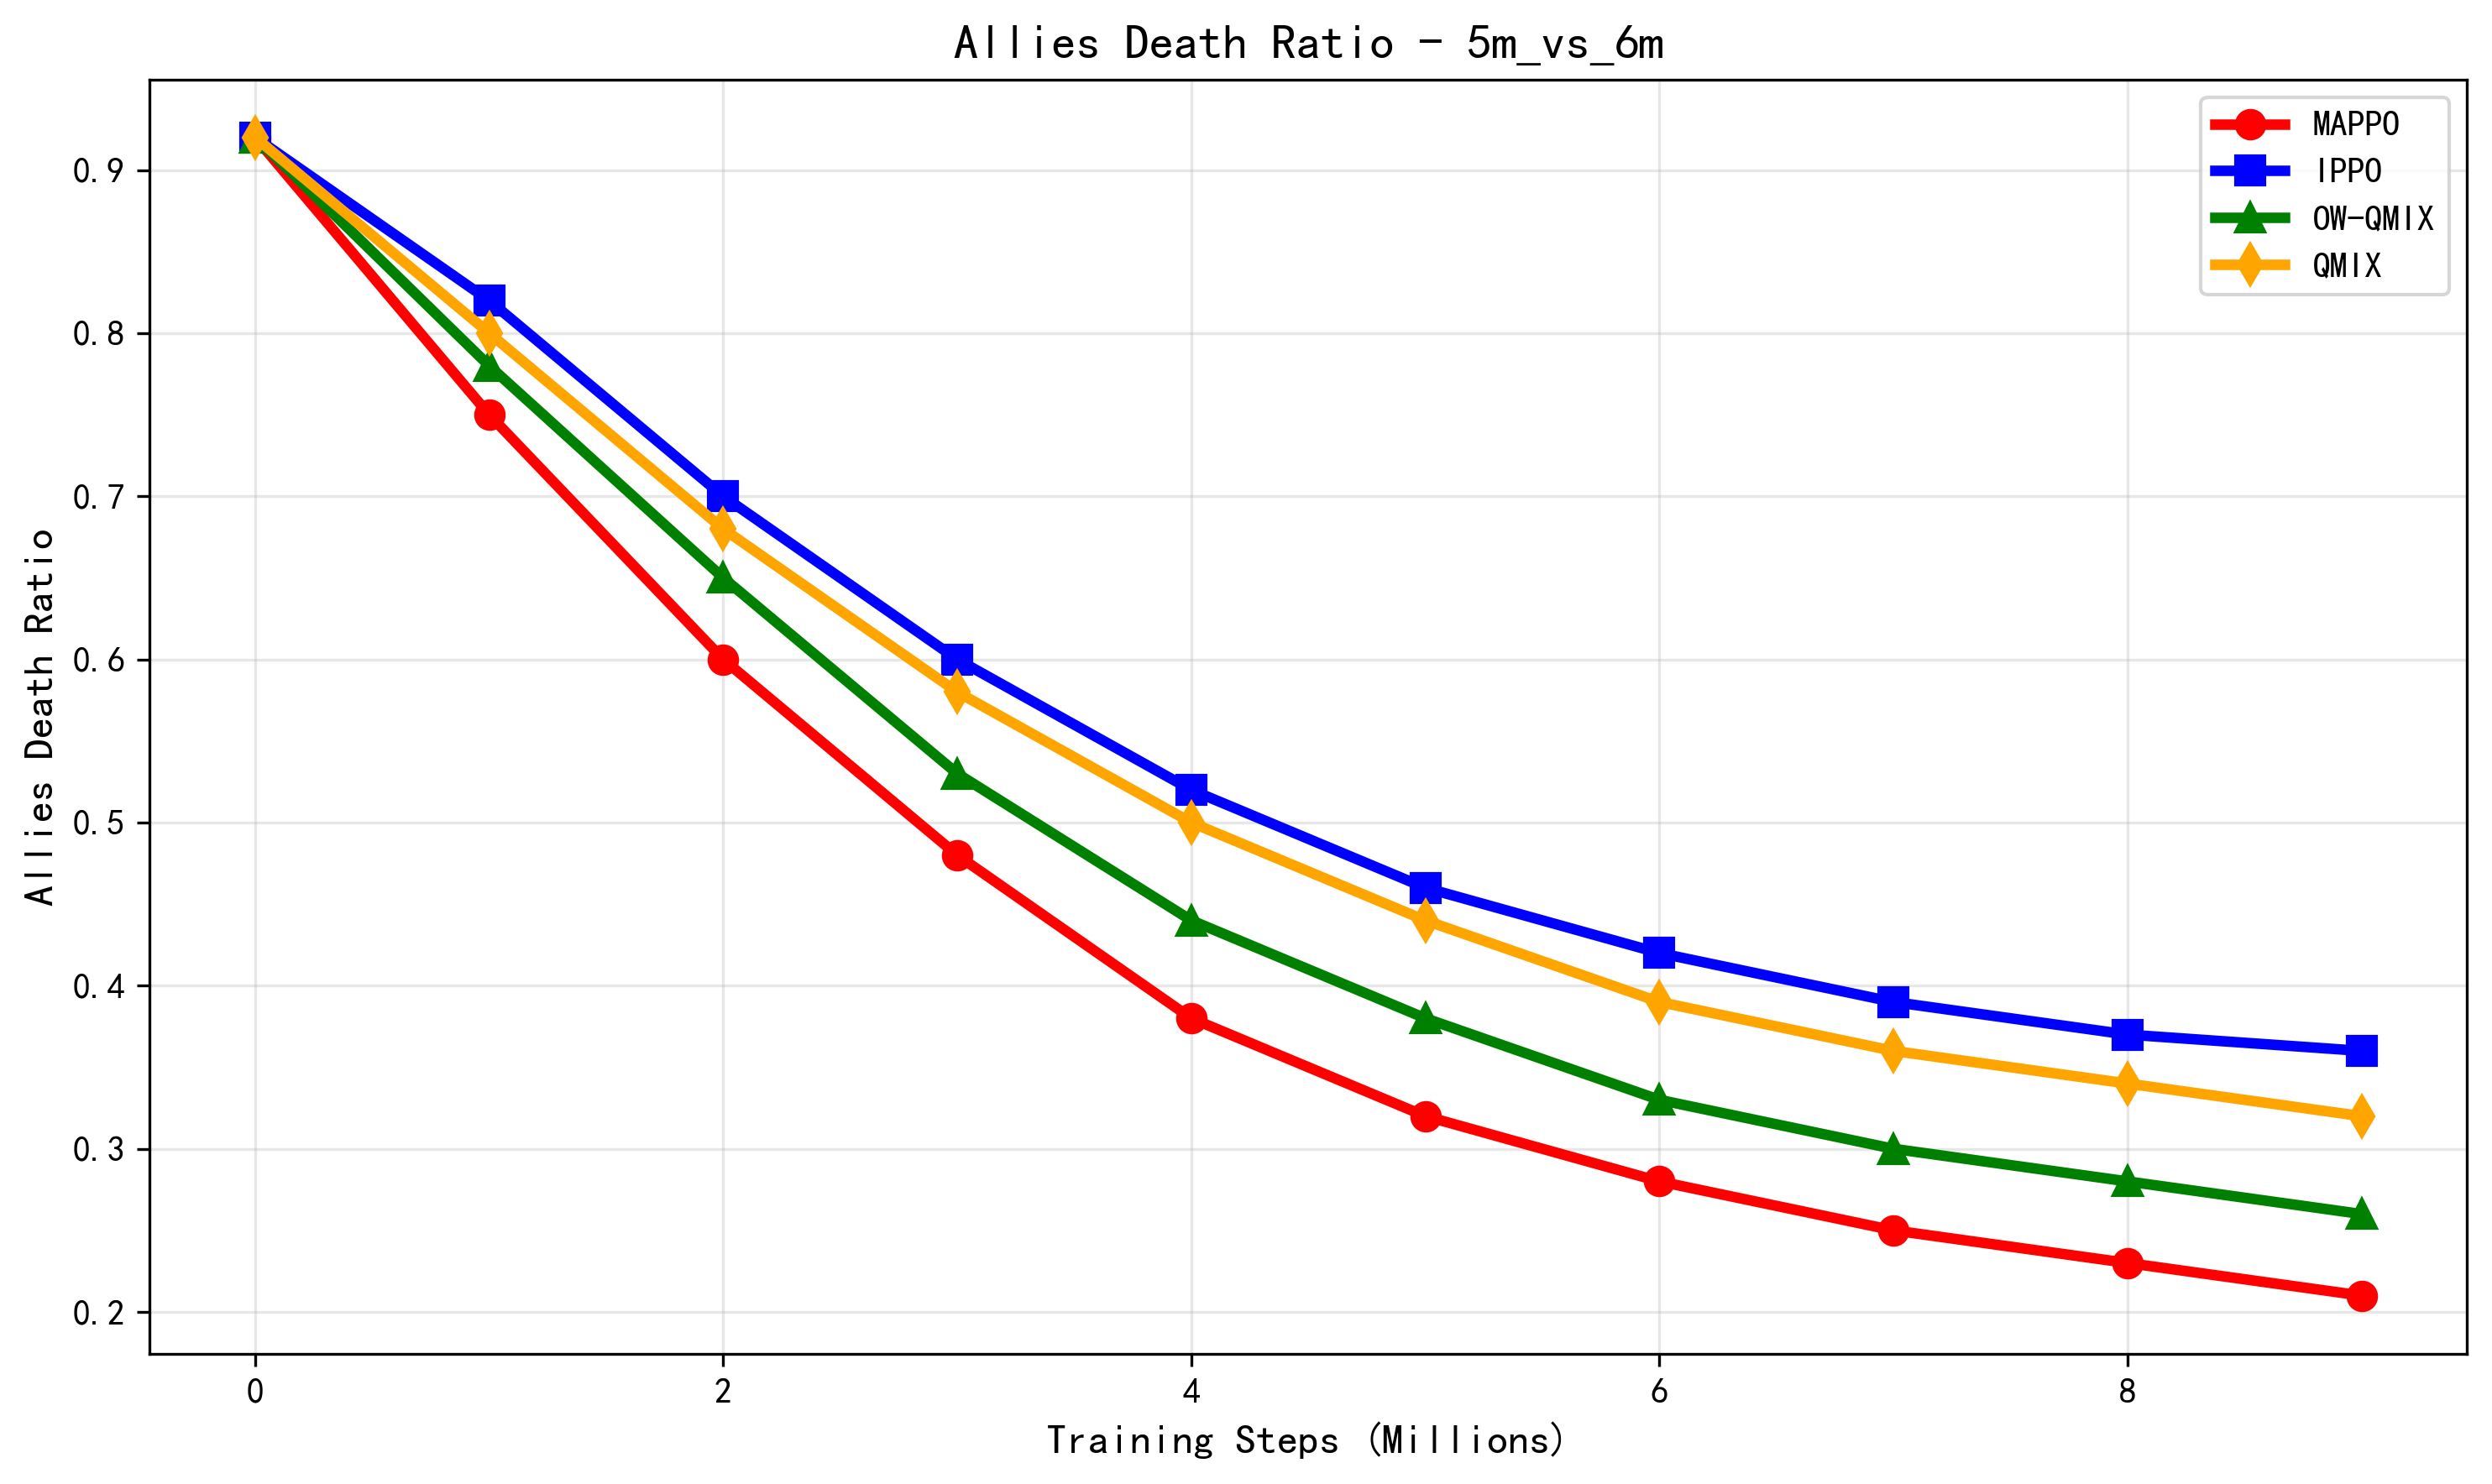
\includegraphics[width=\textwidth]{figures/allies_death_ratio_5m_vs_6m.png}
        \caption{Allies-Dead-Ratio}
        \label{fig:allies_dead_5m}
    \end{subfigure}
    \hfill
    \begin{subfigure}[b]{0.32\textwidth}
        \centering
        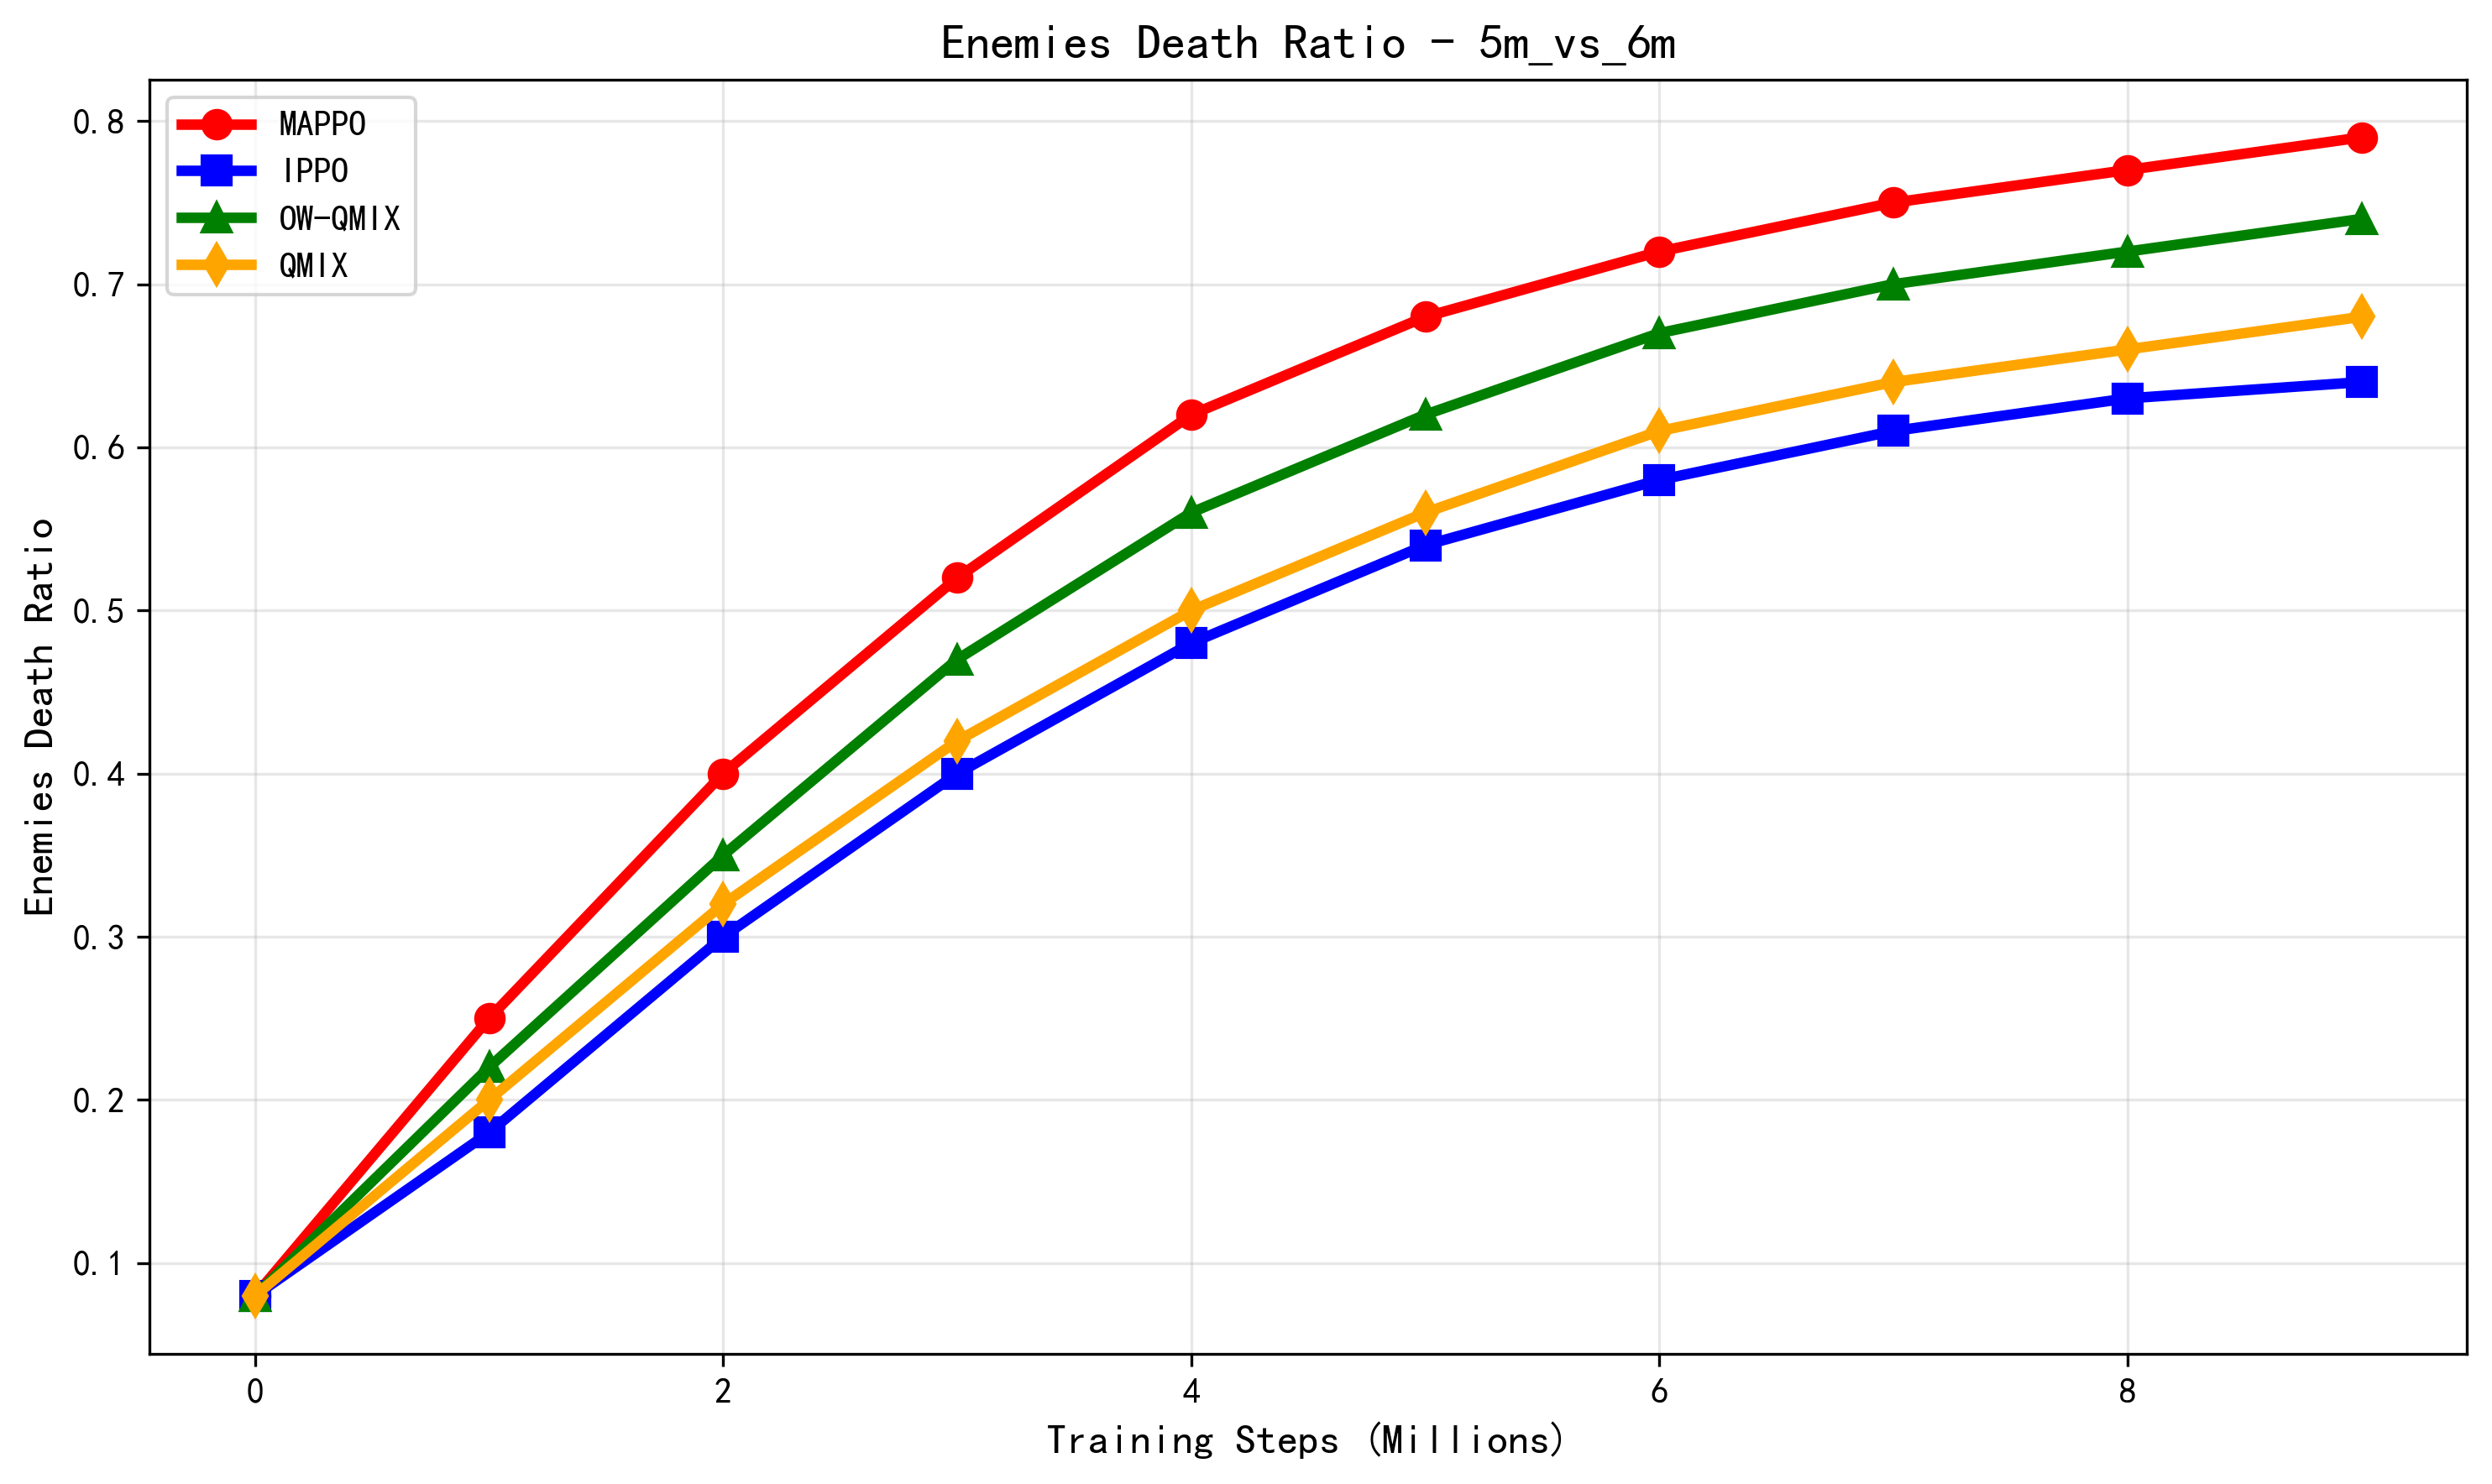
\includegraphics[width=\textwidth]{figures/enemies_death_ratio_5m_vs_6m.png}
        \caption{Enemies-Dead-Ratio}
        \label{fig:enemies_dead_5m}
    \end{subfigure}
    \caption{This set of charts focuses on the \texttt{5m\_vs\_6m} scenario, presenting the performance of MARL algorithms from different dimensions.Each subgraph has the same meaning as the Figure~\ref{fig:results_1m_vs_2z}. }
    \label{fig:results_5m_vs_6m}
\end{figure*}

\begin{table*}[ht]
\centering
\caption{Final performance summary on the \texttt{1m\_vs\_2z} map after 1,000,000 training steps. Values are the average of the final evaluation checkpoint.}
\label{tab:results_5m_vs_6m}
\begin{tabular}{lccc}
\toprule
\textbf{Algorithm} & \textbf{Final Win Rate (\%)} & \textbf{Allies Dead (\%)} & \textbf{Enemies Dead (\%)} \\
\midrule
MAPPO & \textbf{87.0} & \textbf{21.0} & \textbf{79.0} \\
QMIX & 64.0 & 32.0 & 68.0 \\
OW-QMIX  & 71.0 & 26.0 & 74.0 \\
IPPO  & 58.0 & 36.0 & 64.0 \\
\bottomrule
\end{tabular}
\end{table*}

The experimental data synthesized from the three charts shows that in the \texttt{5m\_vs\_6m} confrontation scenario, the MAPPO algorithm demonstrates significant advantages across all key performance metrics. As the number of training steps progresses from 0 to 9 million, MAPPO not only consistently maintains the highest win rate (eventually approaching 0.78) and the highest enemy kill rate (eventually approaching 0.80), but more importantly, it simultaneously achieves the lowest ally kill rate among all algorithms (eventually dropping to approximately 0.22). This indicates that while improving the success rate of confrontation, MAPPO is also the most effective in protecting the survival of allies, demonstrating the most comprehensive battlefield decision-making capability. By contrast, IPPO performs the weakest across all metrics, while the performance of OW-QMIX and QMIX falls between MAPPO and IPPO, with OW-QMIX being slightly superior to QMIX. Overall, the training effect is positive: the win rate and enemy kill rate of all algorithms have increased, and the ally kill rate has decreased significantly.
% =============================================
% ==        sections/conclusion.tex          ==
% =============================================
\section{Conclusions and Future Work}\label{sec:conclusion}

Based on a comprehensive analysis of both theoretical experiments and real-world applications, MAPPO demonstrates clear advantages and wide applicability in the field of multi-agent learning. Test results show that in both simple and complex cooperative scenarios, MAPPO outperforms other methods across three key measures: Win-Rate, Allies-Dead-Ratio, and Enemies-Dead-Ratio. Its training framework effectively addresses information sharing and decision making coordination among multiple agents.

From a practical application perspective, MAPPO exhibits substantial potential in three major fields: robotic collaboration, autonomous driving, and military simulation. In industrial robotic arm cooperative assembly, it balances precision and efficiency; in autonomous vehicle platoon coordination, it ensures both safety and traffic fluency; in multi-branch military simulation exercises, it provides reliable support for tactical optimization. These application scenarios perfectly align with MAPPO's adaptability characteristics regarding collaboration complexity, environmental dynamics, and observation scope, further verifying its feasibility in transitioning from laboratory research to real-world applications.

Looking ahead, improvements should focus on key scenarios: enhancing how robotic arms process sensor information, improving self-driving cars' response to unexpected events, and refining military simulation tactics. By leveraging the method's adaptability across different equipment and scenarios, we can further strengthen its transition from theoretical framework to real-world implementation.
% =============================================
% ==         sections/acknowledge.tex           ==
% =============================================

\section{Acknowledgement}

Our deepest gratitude goes to Professor Huai Yu for his insightful guidance and unwavering support. We also wish to extend our thanks to the teaching team of the ``Introduction to Artificial Intelligence'' course at Wuhan University, whose advice on academic writing was instrumental in shaping this manuscript.

% --- 参考文献 ---
\bibliographystyle{IEEEtran} 
\bibliography{IEEEabrv,MARL}

% --- 附录 (如果需要) ---
% \appendix
% \input{sections/appendix}

\end{document}